 % !TEX root = main.tex
%   Filename    : main.tex
%   Description : This is the main file for the LaTeX thesis proposal document template.
%  Filename   : preamble.tex
%  Description: Preamble file to :
%               a. specify related packages
%               b. set margins, commands, etc.
%\documentclass[12pt,titlepage,onepage, letterpaper]{article}
\documentclass[12pt,titlepage,onepage, letterpaper]{report}
%
%-- specify related packages
% \usepackage[utf8x]{inputenc}
\usepackage{pdfpages}
\usepackage{apacite}         %-- APA style citation  http://www.ctan.org/tex-archive/biblio/bibtex/contrib/apacite/
\usepackage{amsmath}       % American Math Society packages
\usepackage{amsfonts}
\usepackage{amssymb}
\usepackage{graphicx}      %needed for including figures in JPG or PNG format
\usepackage{verbatim}     % tmultiple lines of comments
                               %-- example:
                               %   \begin{comment}
                               %        ...your text here...
                               %   \end{comment}  
\usepackage{color}  %-- allows use of color with text
                               %-- example:  \textcolor{red}{This is the colored text in red.}
\usepackage{url}  %-- allows use of URLs example: \url{https:\ccs1.dlsu.edu.ph}

\usepackage{adjustbox}

\usepackage{lineno}
\usepackage{float}
\usepackage{subfig}


%
%-- set margins,  you may need to edit this for your own printer
%
\topmargin 0.0in
\oddsidemargin 0.0in
\evensidemargin 0.0in

\voffset 0.0in
\hoffset 0.5625in

\textwidth 5.75in
\textheight 8.5in


\parskip 1em
\parindent 0.25in
\bibliographystyle{apacite}            %-- use APA citation scheme
\hyphenation{ana-lysis know-ledge}     %-- LaTeX may not hyphenate correctly some words you use in your document
                                       %-- use \hyphenation to instruct LaTeX how to do it correctly, example above
\newcommand{\degree}{^{\circ}}         %-- use \newcommand to create your own "commands"
\newcommand{\etal}{et al.}
\newcommand{\figref}[1]{Figure \ref{#1}}
\newcommand{\appref}[1]{Appendix \ref{#1}}

\usepackage{comment} % to use the comment environment
\usepackage{titlesec}

\setcounter{secnumdepth}{4}
\usepackage[utf8]{inputenc}
\usepackage{array}
%\usepackage{mathptmx} % tnr
%\newcommand{\Section}[1]{\section{#1}\setcounter{figure}{0}\setcounter{table}{0}}

%\newcommand{\shade}{\multicolumn{1}{|>{\columncolor[gray]{0.25}}c|}{}}
%\newcommand{\tableheader}[1]{\rowcolor{black}\color{white}{#1}}
%\newcommand{\cell}[2]{\multicolumn{1}{#1}{#2}}
%\newcommand{\definition}[2]{\textbf{\textit{#1}} --- #2}
%\newcommand{\itembit}[1]{\item \textbf{\textit{#1}}}
%\newcommand{\sgdef}[2]{\parbox[t][][t]{1.75in}{\textbf{#1}} \> \parbox[t][][t]{4.0in}{#2}\\\\}

%\newenvironment{sinagglossary}{\begin{flushleft}
%\begin{tabbing}
%\hspace{1.75in}\=\\}{\end{tabbing}\end{flushleft}}

\newcommand{\thestitle}[1]{{\Large \textsc{#1}}}


%---
%  \renewcommand{\thefigure}{\thesection.\arabic{figure}}
%  \renewcommand{\thetable}{\thesection.\arabic{table}}
%  \renewcommand{\contentsname}{Table of Contents}

\newcommand{\weektwo}{\textbf{W2}}    % Example for Week 2
\newcommand{\weekthree}{\textbf{W3}}  % Example for Week 3
\newcommand{\weekfour}{\textbf{W4}}   % Example for Week 4
\newcommand{\weekone}{\textbf{W1}}    % Example for Week 1
\usepackage{pdflscape}
\usepackage{caption}     
\graphicspath{{figures/}}  %figures is the name of the folder containing images JPG or PNG

\begin{document}
\linenumbers
%   Filename    : title_page.tex 
\begin{titlepage}
\centering

%-- **EDIT** the following line to indicate your thesis title
\thestitle{Road Defect Severity Assessment  and Classification}

\vspace{1.75cm}
A Special Problem Proposal\\
Presented to\\
the Faculty of the Division of Physical Sciences and Mathematics\\
College of Arts and Sciences\\
University of the Philippines Visayas\\
Miag-ao, Iloilo

\vspace{1.75cm}
In Partial Fulfillment\\
of the Requirements for the Degree of\\
Bachelor of Science in Computer Science
\vspace{1.75cm}
by\\

\vspace{1cm}
% list in alphabetical order by lastnames
BELEBER, Benz Vrianne  \\
CATALAN, Perserose  \\
SENCIL, Kristian Lyle  \\
% LASTNAME4, FirstName4  \\

\vspace{1.75cm}
Francis DIMZON, Ph.D. \\
Adviser\\

\vspace{1.75cm}
\today
\end{titlepage}
      %includes LaTeX source file for the Title Page 
\pagenumbering{roman}   %number pages as i, ii, iii, etc...
\setcounter{page}{2}
%   Filename    : approval.tex 
\begin{center}
	\textbf{Approval Sheet}
	
	The Division of Physical Sciences and Mathematics, College of Arts and Sciences, University of the Philippines Visayas 
	
	certifies that this is the approved version of the following special problem:
	
	\thestitle{Road Defect Severity Assessment  and Classification}
\end{center}

{\small\textbf{Approved by:}}

\newcommand{\signaturerule}{\rule{10em}{.4pt}}
\begin{tabular}{lll}
	\bfseries Name  & \bfseries Signature & \bfseries Date\\ \\
	Francis D. Dimzon, Ph.D. &\signaturerule  & \signaturerule\\ 
	\multicolumn{1}{l}{(Adviser)} \\ 
	Ara Abigail E. Ambita &\signaturerule &\signaturerule\\
	\multicolumn{1}{l}{(Panel Member)}  \\
	Kent Christian A. Castor &\signaturerule &\signaturerule\\
	\multicolumn{1}{l}{(Division Chair)}
	
\end{tabular}

%   Filename    : declaration.tex 
\begin{center}
	Division of Physical Sciences and Mathematics\\
	College of Arts and Sciences\\
	University of the Philippines Visayas 
	
	\textbf{Declaration}
\end{center}

We,  {BENZ VRIANNE BELEBER}, {PERSEROSE CATALAN}, and {KRISTIAN LYLE SENCIL}, hereby certify that this Special Problem has been written by us  and is the record of work carried out by us. Any significant borrowings have been properly acknowledged and referred.

\begin{tabular}{lll}
	\bfseries Name  & \bfseries Signature & \bfseries Date\\ \\
	Benz Vrianne Beleber &\signaturerule  & \signaturerule\\ 
	\multicolumn{1}{l}{(Student)} \\ 
	Perserose Catalan &\signaturerule  & \signaturerule\\ 
	\multicolumn{1}{l}{(Student)} \\
	Kristian Lyle Sencil &\signaturerule  & \signaturerule\\ 
	\multicolumn{1}{l}{(Student)} \\
	
\end{tabular}

%   Filename    : dedication.tex 
\begin{center}
	\textbf{Dedication}
\end{center}

\vspace{2em}

This Special Problem is dedicated to the researchers’ families, whose unwavering love, patience, and support have been the foundation of their academic journey.

To their parents, for their endless sacrifices.

To their mentors and teachers, for believing in them and guiding them with wisdom.

And to all those who inspired them to keep going even in the most challenging moments — this work is for them.
\begin{center}
	\textbf{\Large Acknowledgment}
\end{center}

\vspace{2em}

The researchers would like to express their heartfelt gratitude to the individuals, institutions, and organizations who made the completion of this Special Problem possible:

To their adviser, Dr. Francis Dimzon, for his expert guidance, valuable insights, for teaching Computer Vision topics, and unwavering support throughout the research process.

To Prof. Jumar Cadondon, for lending his time and expertise during the early stages of this Special Problem, especially in providing assistance with his drone.

To Sir Cris Beleber, for his unwavering support from the initial conceptualization of this project to out consultations with the DPWH. His assistance was instrumental in the successful completion of this study.

To the Komsai faculty and staff, for providing a nurturing and intellectually stimulating environment.

To the university personnel who ensured the researchers' safety throughout the data collection process.

To the Department of Science and Technology (DOST), for their support and promotion of scientific research and innovation.

To the Department of Public Works and Highways (DPWH), for providing valuable data and technical insights that greatly contributed to the relevance and application of the study.

To their families and friends, for their unconditional love, patience, and encouragement.

Lastly, to the University of the Philippines Visayas, for providing the resources and environment necessary for the researchers to explore and grow.

This work stands as a testament to the collaboration, support, and trust the researchers have received. They are deeply grateful.
%   Filename    : abstract.tex 
\begin{center}
\textbf{Abstract}
\end{center}
\setlength{\parindent}{0pt}
Road surveying is a crucial part of the maintenance processes of roads in the Philippines that is carried out by the Department of Public Works and Highways. However, the current process of road surveying is time consuming which delays much needed maintenance operations. Existing studies involving automated pothole detection lack integration of the pothole's depth in assessing its severity which is essential for automating road  surveying procedures.  A system that incorporates estimated depth information in assessing pothole severity is developed in order to automate the manual process of depth measurement and severity assessment in road surveying. For depth estimation, stereo vision is favorable in this context as depth may be estimated through the disparity generated by a stereo pair. In obtaining a stereo view of the potholes, the StereoPi V2 is utilized along with some modifications that would make it eligible for outdoor use.
To address camera imperfections, a fitted inverse model was applied to improve the accuracy of depth estimates. Linear regression analysis revealed a strong positive correlation (R = 0.978) between estimated and actual depths, with the system measuring pothole depths mostly within 3 cm of the true values.

%  Do not put citations or quotes in the abract.

\begin{tabular}{lp{4.25in}}
\hspace{-0.5em}\textbf{Keywords:}\hspace{0.25em} & pothole, depth estimation, stereo vision, StereoPi V2\\
\end{tabular}
   %number pages as i, ii, iii, etc...
\setcounter{page}{2}
\tableofcontents                  %generate the Table of Contents
\newpage
\listoffigures                    %generate List of Figures
\newpage                       
\listoftables                     %generate List of Tables
\newpage
\pagenumbering{arabic}            %number pages as 1, 2, 3, etc...
\setcounter{page}{1}              
%   Filename    : chapter_1.tex 
\chapter{Introduction}
\label{sec:researchdesc}    %labels help you reference sections of your document

\section{Overview}
\label{sec:overview}
According to the National Road Length by Classification, Surface Type, and Condition of the Department of Public Works and Highways (DPWH), as of October 2022 approximately 98.97% of roads in the Philippines is paved which is either made of concrete or asphalt (DPWH, 2022)(?). Since the DPWH is an institution under the government, it is paramount to maintain such roads in order to avoid accidents and congested traffic situations especially in heavily urbanized areas where there are a lot of vehicles.


In an interview with the Road Board of DPWH Region 6 it was stated that road condition assessments are mostly done manually with heavy reliance on engineering judgment. In addition, manual assessment of roads is also time consuming which leaves maintenance operations to wait for lengthy assessments (J. Chua, Personal Interview. 16 September 2024).  In a study conducted by Ramos, Dacanay, and Bronuela-Ambrocio (2022), it was found that the Philippines’ current method of manual pavement surveying is considered as a gap since it takes an average of 2-3 months to cover a 250 km road as opposed to a 1 day duration in the Australian Road Research Board for the same road length. Ramos et al. (2022) recommended that to significantly improve efficiency of surveying methods and data gathering processes, automated survey tools are to be employed. It was also added that use of such automated surveying tools can also guarantee the safety of road surveyors (Ramos et al., 2022).


If the process of assessment on the severity of road defects can be automated then the whole process of assessing the quality of roads can be hastened up which can also enable maintenance operations to commence as soon as possible if necessary. If not automated, the delay of assessments will continue and roads that are supposedly needing maintenance may not be properly maintained which can affect the general public that is utilizing public roads daily.


\section{Problem Statement}
Roads support almost every aspect of daily life, from providing a way to transport goods and services to allowing people to stay connected with their communities. However, road defects such as cracks and potholes damage roads over time, and they can increase accident risks and affect the overall transportation. The current way of inspecting the roads for maintenance is often slow as it is done manually, which makes it harder to detect and fix defects early. The delay in addressing these problems can lead to even worse road conditions (J. Chua, Personal Interview. 16 September 2024). There are several research studies into automated road defect classification that have advanced in recent years but most of them focus on identifying the types of defects rather than assessing their severity or characteristics like depth. Without reliable data on the depth of the defect, road maintenance authorities may underestimate the severity of certain defects. To address these challenges, advancements are needed across various areas. An effective solution should not only detect and classify road defects but also measure their severity to better prioritize repairs. Failing to address this problem will require more extensive repairs for damaged roads, which raises the cost and strains the budget. Additionally, road maintenance would still be slow and cause disruptions in daily activities. Using an automated system that accurately detects, classifies, and assess the severity of road defects by incorporating depth are necessary to efficiently monitor road quality.


\section{Research Objectives}
\label{sec:researchobjectives}

\subsection{General Objective}
\label{sec:generalobjective}

This special problem aims to develop an automated system that will accurately detect, classify, and assess the severity of the different types of road defects by using image analysis, depth measurement technologies, and combination of machine learning and computer vision techniques. 



\subsection{Specific Objectives}
\label{sec:specificobjectives}

Specifically, this special problem aims:
\begin{enumerate}
   \item To collect high-quality images of road surfaces that capture different types of road defects including their depth in various lighting and weather conditions.
   \item To develop and train a machine learning model to detect, classify, and assess the severity of road defects from images. 
   \item To measure the accuracy of the system by comparing the depth measurements against ground truth data collected from actual road inspections
   \item To develop a prototype system that can detect and measure road defects from image input, analyze their depth, and assess their severity.
\end{enumerate}


\section{Scope and Limitations of the Research}
\label{sec:scopelimitations}



This system will include a collection of images of  different road defects, such as potholes and cracks, using cameras and depth-sensing tools. The images will be captured under various lighting and weather conditions to ensure that the data has variations. The scope is limited to visual and depth data. High-quality and diverse  image data sets are essential for training an efficient model, and by focusing on capturing the depth, it will allow a more accurate assessment of severity of the road defects. 


Depth measurement tools, such as LiDAR drones or stereo cameras will be used to record the depth of the road defect. Only accessible defects will be measured, any cracks and potholes filled with water may not be accurately assessed. 


A machine learning model will be used to identify, classify, and assess the severity of road defects. It will use the image dataset to classify and assess the road defect types accurately, however, the effectiveness will depend on the quality and quantity of the training dataset. There can be a limited variety of images or inaccuracies due to environmental factors. The model will allow consistent and automated assessment of road defects which is more efficient than manual inspection. 


The accuracy of the system will be evaluated by comparing the depth measurement it produces against data collected from the field through manual inspections. However, the comparisons could be limited to selected sample sites because collecting field data across a wide area can be time-consuming. Comparing the data is important to validate the reliability of the system. It ensures that the data that the system produces is accurate so it increases confidence in using it for road maintenance. 


\section{Significance of the Research}
\label{sec:significance}

This special problem aims to be significant to the following:


\textit{Computer Science Community}. This system can contribute to advancements in computer vision and machine learning by using both visual and depth data to assess the severity of road defects. It introduces a more comprehensive approach compared to the usual image-only or manual inspection methods. This combination can be applied to other fields that need both visual and depth analysis like medical imaging. 


\textit{Concerned Government Agencies.} This system offers a valuable tool for road safety and maintenance. Not only can this detect and classify anomalies, it can also assess the defect’s severity which allows them to prioritize repairs, optimal project expenditures, and better overall road safety and quality. 


\textit{Field Engineers.} In the scorching heat, field engineers are no longer required to be on foot unless it requires its engineering judgement when surveying a road segment. It can hasten the overall assessment process. 


\textit{Future Researchers.} The special problem can serve as a baseline and guide of researchers with the aim to pursue special problems similar or related to this. 


               %LaTeX source file for Chapter 1: Introduction
%   Filename    : chapter_2.tex 
\chapter{Review of Related Literature}

\section{Frameworks}
This section of the chapter presents related literature that is considered essential for the development of this special problem.

\subsection{Depth Estimation}
Depth estimation as defined by \citeA{sanz2012} as a set of processes that aims to extract a representation of a certain scene's spatial composition. Stereo vision is stated to be among the depth estimation strategies \cite{sanz2012}.

\subsection{Image and Video Processing}
\citeA{kumar2024} defines image processing as a process of turning an image into its digital form and extracting data from it through certain functions and operations. Usual processes are considered to treat images as 2D signals wherein different processing methods utilize these signals.
Like image processing, \citeA{riches2020} defines video processing as being able to extract information and data from video footage through signal processing methods. However, in video processing due to the diversity of video formats, compression and decompression methods are often expected to be performed on videos before processing methods to either increase or decrease bitrate.

\subsection{Stereo Vision}
MathWorks (n.d.) defines stereo vision as a process of utilizing multiple 2D perspectives in order to extract information in 3D. In addition, most uses of stereo vision involve estimating an objects distance from an observer or camera. The 3D information is stated to be extracted with stereo pairs or pair of images through estimation of relative depth of points in a scene which are then represented through a stereo map that is made through the matching of the pair's corresponding points.


\section{Related Studies}
This section of the chapter presents related studies conducted by other researchers wherein the methodology and technologies used may serve as basis in the development of this special problem.

\subsection{Deep Learning Studies}

\subsubsection{Automated Detection and Classification of Road Anomalies in VANET Using Deep Learning}
In the study of Bibi et al. (2021) it was noted that identification of active road defects are critical in maintaining smooth and safe flow of traffic. Detection and subsequent repair of such defects in roads are crucial in keeping vehicles using such roads away from mechanical failures. The study also emphasized the growth in use of autonomous vehicles in research data gathering which is what the researchers utilized in data gathering procedures. With the presence of autonomous vehicles, this allowed the researchers to use a combination of sensors and deep neural networks in deploying artificial intelligence. The study aimed to allow autonomous vehicles to avoid critical road defects that can possibly lead to dangerous situations. Researchers used Resnet-18 and VGG-11 in automatic detection and classification of road defects. Researchers concluded that the trained model was able to perform better than other techniques for road defect detection \cite{bibi2021}. The study is able to provide the effectiveness of using deep learning models in training artificial intelligence for road defect detection and classification. However, the study lacks findings regarding the severity of detected defects which is crucial in automating manual procedures of road surveying in the Philippines.

\subsubsection{Road Anomaly Detection through Deep Learning Approaches}
The study of \citeA{luo2020} aimed to utilize deep learning models in classifying road anomalies. The researchers used three deep learning approaches namely Convolutional Neural Network, Deep Feedforward Network, and Recurrent Neural Network from data collected through the sensors in the vehicle's suspension system. In comparing the performance of the three deep learning approaches, the researchers fixed some hyperparameters. Results revealed that the RNN model was the most stable among the three and in the case of the CNN and DFN models, the researchers suggested the use of wheel speed signals to ensure accuracy. And lastly, the researchers concluded that the RNN model was best due to high prediction performance with small set parameters \cite{luo2020}.

\subsubsection{Assessing Severity of Road Cracks Using Deep Learning-Based Segmentation and Detection}
In the study of \citeA{ha2022}, it was argued that the detection, classification, and severity assessment of road cracks should be automated due to the bottleneck it causes during the entire process of surveying. For the study, the researchers utilized SqueezNet, U-Net, and MobileNet-SSD models for crack classification and severity assessment. Furthermore, the researchers also employed separate U-nets for linear and area cracking cases. For crack detection, the researchers followed the process of pre-processing, detection, classification. During preprocessing images were smoothed out using image processing techniques. The researchers also utilized YOLOv5 object detection models for classification of pavement cracking wherein the YOLOv51 model recorded the highest accuracy. The researchers however stated images used for the study are only 2D images which may have allowed higher accuracy rates. Furthermore, the researchers suggest incorporating depth information in the models to further enhance results.

\subsubsection{Roadway pavement anomaly classification utilizing smartphones and artificial intelligence}
The study of \citeA{kyriakou2016} presented what is considered as a low-cost technology which was the use of Artificial Neural Networks in training a model for road anomaly detection from data gathered by smartphone sensors. The researchers were able to collect case study data using two-dimensional indicators of the smartphone’s roll and pitch values. In the study’s discussion, the data collected displayed some complexity due to acceleration and vehicle speed which lead to detected anomalies being not as conclusive as planned. The researchers also added that the plots are unable to show parameters that could verify the data’s correctness and accuracy. Despite the setbacks, the researchers still fed the data into the Artificial Neural Network that was expected to produce two outputs which were “no defect” and “defect.” The method still yielded above 90\% accuracy but due to the limited number of possible outcomes in the data processing the researchers still needed to test the methodology with larger data sets and roads with higher volumes of anomalies.

\subsection{Machine Learning Studies}

\subsubsection{Smartphones as Sensors for Road Surface Monitoring}
In their study, \citeA{sattar2018} noted the rise of sensing capabilities of smartphones which they utilized in monitoring road surface to detect and identify anomalies. The researchers considered different approaches in detecting road surface anomalies using smartphone sensors. One of which are threshold-based approaches which was determined to be quite difficult  due to several factors that are affecting the process of determining the interval length of a window function in spectral analysis \cite{sattar2018}. The researchers also utilized a machine learning approach adapted from another study. It was stated that k-means was used in classifying sensor data and in training the SVM algorithm. Due to the requirement of training a supervised algorithm using a labeled sample data was required before classifying data from sensors, the approach was considered to be impractical for real-time situations \cite{sattar2018}. In addition, \citeA{sattar2018} also noted various challenges when utilizing smartphones as sensors for data gathering such as sensors being dependent on the device’s placement and orientation, smoothness of captured data, and the speed of the vehicle it is being mounted on. Lastly, it was also concluded that the accuracy and performance of using smartphone sensors is challenging to compare due to the limited data sets and reported algorithms.

\subsubsection{Road Surface Quality Monitoring Using Machine Learning Algorithms}
The study of \citeA{singh2021} aimed to utilize machine learning algorithms in classifying road defects as well as predict their locations. Another implication of the study was to provide useful information to commuters and maintenance data for authorities regarding road conditions. The researchers gathered data using various methods such as smartphone GPS, gyroscopes, and accelerometers. \cite{singh2021} also argued that early existing road monitoring models are unable to predict locations of road defects and are dependent on fixed roads and static vehicle speed.  Neural and deep neural networks were utilized in the classification of anomalies which was concluded by the researchers to yield accurate results and are applicable on a larger scale of data \cite{singh2021}. The study of \citeA{singh2021} can be considered as an effective method in gathering data about road conditions. However, it was stated in the study that relevant authorities will be provided with maintenance operation and there is no presence of any severity assessment in the study. This may cause confusion due to a lack of assessment on what is the road condition that will require extensive maintenance or repair.

\subsection{Computer Vision Studies}

\subsubsection{Stereo Vision Based Pothole Detection System for Improved Ride Quality}
In the study of \citeA{ramaiah2021} it was stated that stereo vision has been earning attention due to its reliable obstacle detection and recognition. Furthermore, the study also discussed that such technology would be useful in improving ride quality in automated vehicles by integrating it in a predictive suspension control system. The proposed study was to develop a novel stereo vision based pothole detection system which also calculates the depth accurately. However, the study focused on improving ride quality by using the 3D information from detected potholes in controlling the damping coefficient of the suspension system. Overall, the pothole detection system was able to achieve 84\% accuracy and is able to detect potholes that are deeper than 5 cm. The researchers concluded that such system can be utilized in commercial applications. However, it is also worth noting that despite the system being able to detect potholes and measure its depth, the overall severity of the pothole and road condition was not addressed.

\newpage
\section{Chapter Summary}
The reviewed literature involved various techniques and approaches in  road anomaly detection and classification. These approaches are discussed and summarized below along with their limitations and research gaps.
\begin{table}[h!]
	\centering
	\hspace{-2cm}
	\small 
	\begin{tabular}{|p{3cm}|p{3.5cm}|p{4.5cm}|p{4.5cm}|}
		\hline
		\textbf{Study} & \textbf{Technology/
			Techniques Used} & \textbf{Key Findings} & \textbf{Limitations} \\ \hline
		
		Automated Detection and Classification of Road Anomalies in VANET Using Deep Learning & Resnet-18 and VGG-11 & Trained model is able to provide the effectiveness of using deep learning models in training artificial intelligence for road defect detection and classification. & Lacks findings regarding the severity of detected defects. \\ \hline
		
		Smartphones as sensors for Road surface monitoring & Machine Learning, Smartphones & Approach was considered impractical for real-life applications. & Sensors are dependent on device's placement and orientation, smoothness of data, and speed of vehicle it is mounted on. Accuracy of results is difficult to compare. \\ \hline
		
		Road Anomaly Detection through Deep Learning Approaches & Convolutional Neural Network, Deep Feedforward Network, and Recurrent Neural Network & Identified that RNN was the best deep learning approach due to high prediction performance. & Data collection is considered too difficult and complicated to execute due to sensors being mounted on an integral part of the vehicle. \\ \hline
		
		Assessing Severity of Road Cracks Using Deep Learning-Based Segmentation and Detection & SqueezNet, U-Net, YOLOv5, and MobileNet-SSD models & YOLOv51 model recorded the highest accuracy. & Only 2D images are used for the study which may have allowed higher accuracy rates, and the study also lacked depth information. \\ \hline
		
		Stereo Vision Based Pothole Detection System for Improved Ride Quality & Pair of stereo images captured by a stereo camera & System was able to achieve 84\% accuracy and is able to detect potholes that are deeper than 5 cm. & Overall severity of the pothole and road condition was not addressed. \\ \hline
		
	\end{tabular}
	\caption{Comparison of Related Studies on Road Anomaly Detection using Deep Learning Techniques and Stereo Vision}
	\label{tab:comparison}
	\hspace{-3cm}
\end{table}               %LaTeX source file for Chapter 2: Review of Related Literature
%   Filename    : chapter_3.tex 
\chapter{Research Methodology}
This chapter outlines the systematic approach that were taken to address the problem of pothole depth estimation using StereoPi V2. The methodology is divided into key phases: data collection, algorithm selection, design, testing and experimentation, and challenges and limitations. Each phase will play a crucial role in accurately classifying and assessing road defects.  Each phase is essential for accurately estimating the depth of potholes using StereoPi V2. 

\section{ Research Activities}

\subsection{Data Collection}
The researchers conducted initial inquiries to understand the problem domain and existing road maintenance practices. This phase included consulting the engineers under the Road Maintenance Department of the government agency Department of Public Works and Highways (DPWH). An interview with Engr. Jane Chua provided a comprehensive overview of the DPWH's road maintenance manual, which was crucial in aligning this project with existing standards. This collaboration with DPWH provided insights into road pothole classification standards, ensuring that the collected data will align with industry standards. The DPWH manual primarily focuses on the volume of detected potholes within a road segment as a measure of severity. However, since depth is not explicitly measured in their current procedures, the study will supplement this by referencing international standards such as the Long-Term Pavement Performance (LTPP) classification used in the United States \cite{miller2014}. The LTPP categorizes potholes based on depth thresholds, which will be integrated with DPWH’s volume-based assessment to provide a more comprehensive severity classification framework. The data collection involved capturing around 130 images of potholes from various locations within the UP Visayas Campus. Ground truth data of pothole depth were collected by the researchers by measuring the depth of different points in an individual pothole and then solving for its average depth. The researchers developed a manual specifically designed for depth measurement, which underwent a review by Engr. Benjamin Javellana, Assistant Director of the Maintenance Division at the Department of Public Works and Highways (DPWH) Regional Office VI. The finalized version of the manual was subsequently validated by the DPWH First District Engineering Office. In order to individually locate or determine each pothole where the ground truth data is collected, images taken were labeled with their corresponding coordinates, street names, and nearby landmarks.

\subsubsection{Data Collection (Ground Truth Data)}
Data collection took place between January and March 2025, during which the researchers collected depth information from 130 potholes around the University of the Philippines Visayas Miagao Campus. During data collection, the researchers are equipped with safety vests and an early warning device to give caution to incoming vehicles. Following the validated manual for pothole depth measurement, a ruler and a measuring tape were used in both vertical and horizontal positions as shown in Figure 3.1. This setup helped determine the distance from the road surface to the bottom of the pothole. The researchers recorded four measure points within the pothole as shown in Figure 3.2 and the resulting average is recorded as the pothole's depth.

%pothole manual measure picture%
\begin{center}
	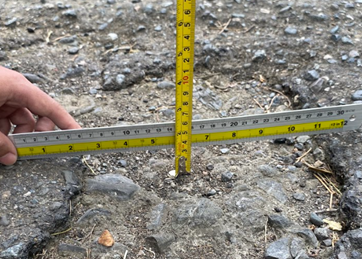
\includegraphics[scale=0.85]{measure.png}
	\captionof{figure}{Manual depth measurement of pothole using a	 ruler and measuring tape.}
\end{center}

%pothole points picture%
\begin{center}
	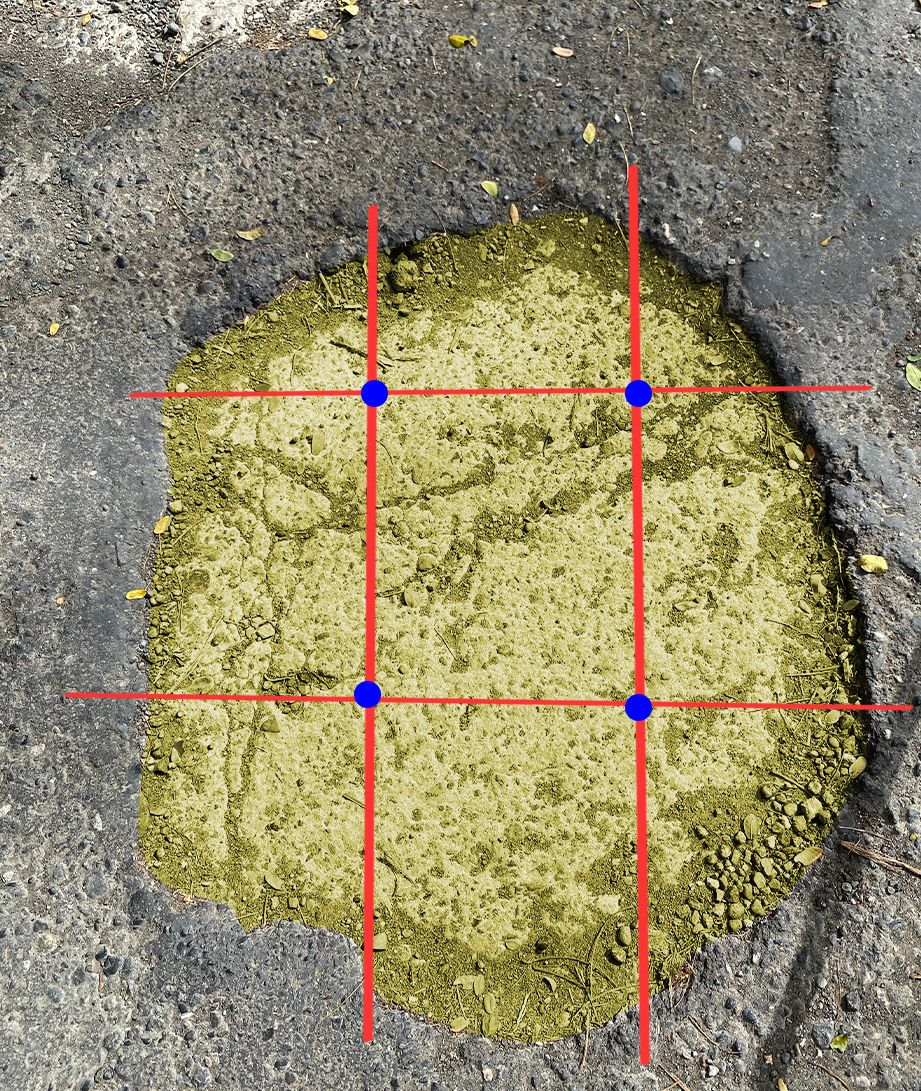
\includegraphics[scale=0.25]{pothole points.jpg}
	\captionof{figure}{Four measure points of the pothole.}
\end{center}

%\subsection{Algorithm Selection} 
%Potential solutions, algorithms, and system architectures were discussed by the researchers and the special problem adviser in this phase. These sessions, conducted in class and virtually via Zoom, helped narrow down the overview of the system, leading to the selection of the main architecture Epipolar Spatio-Temporal Networks (ESTN) for depth estimation. 

%\subsubsection{Pothole Detection}
%YOLOv5 was selected due to its high accuracy and ability to process images in real-time, making it suitable for detecting road defects in dynamic environments. Its architecture is optimized for speed and performance, which is crucial for large-scale deployment in road inspections. 

%\subsubsection{Severity Assessment}
%The Multi-view Depth Estimation using Epipolar Spatio-Temporal Networks was selected due to the high cost and limited accessibility of LiDAR technology. By applying epipolar geometry and temporal consistency across sequential frames, this approach provides an accurate depth estimation from standard video footage \cite{long2021}. 

\subsection{Design, Testing, and Experimentation}
This section outlines both the design and testing of the system, as well as the experimentation process to validate the selected methodologies. 

\subsubsection{Depth Measurement}
Depth estimation is performed by generating disparity maps from the calibrated stereo image pairs captured by the StereoPi V2. In this process, two key measurement points are selected for each pothole: one targeting the pothole area itself, and another targeting the adjacent road surface considered as the reference plane. By calculating the difference in disparity values between these two points, the system estimates the relative depth of the pothole. This approach improves accuracy by normalizing disparity measurements against the nearby road surface, effectively isolating the pothole’s depth from overall scene variation.

The disparity-to-depth conversion utilizes an inverse model derived from calibration data, ensuring that the depth estimates reflect real-world distances accurately within the effective operational range of the stereo camera setup.

\subsubsection{Severity Assessment}

The estimated pothole depths were classified using the Long-Term Pavement Performance (LTPP) depth thresholds, an internationally recognized framework for pavement distress evaluation. This classification provides standardized criteria to assess pothole severity objectively based on measured depth values. Specifically, potholes with depths less than 2.5 cm are categorized as low severity, those between 2.5 cm and 5 cm as medium severity, and potholes exceeding 5 cm are classified as high severity \cite{miller2014}.


%\subsubsection{Model Design}
%The system was designed to operate with two core components: YOLOv5 for pothole detection and ESTN for depth estimation. The model architecture was chosen based on the real-time processing capabilities and the need for accurate depth estimation from standard video footage. The design ensures that the system can detect defects and provide severity assessments in a seamless workflow. 

%\subsubsection{Data Set}
%The YOLOv5 model was trained using two datasets from Universe Roboflow. One of the data sets was posted by a user named Eric Tam. It was also stated that the images from the dataset are sourced from a Crowdensing-based Road Damage Detection Challenge from 2022 in Japan. The challenge involves contestants being required to submit road damage datasets, shortlist their data set, and use the data set for road damage detection and classification models. The use of this data set in training models for road damage detection and classification ensures that the data is viable for training the YOLOv5 model. The dataset contains various road defects in Japan.
%Another data set used in training the YOLOv5 model was also uploaded in Universe Roboflow by a user named Atikur Rahman Chitholian which was stated to be part of his undergraduate thesis. The dataset is comprised of 665 images with potholes being labeled. It was also stated that the data set can be utilized in automatically detecting and categorizing potholes found in the streets of cities.
%Data preprocessing techniques were applied to both datasets to improve model accuracy and generalization. These included resizing images to a uniform size, applying %augmentation techniques (flipping, rotation, and color adjustment) to increase dataset variability, and normalizing pixel values to ensure consistency across images. 
\subsubsection{Materials and Equipment}


The prototype system was constructed using several hardware components, which include the items listed below and shown in Figure 3.3:
\begin{itemize}
	\item StereoPi V2 Board
	\item Raspberry Pi Compute Module 4 (CM4)
	\item Dual RaspberryPi Camera Modules with Fisheye Lens
	\item 3D Printed Custom Housing
	\item 2-inch LCD Module
	\item Micro SD Card
	\item Antenna
	\item Momentary Push Button
\end{itemize}

%Parts picture%
\begin{center}
	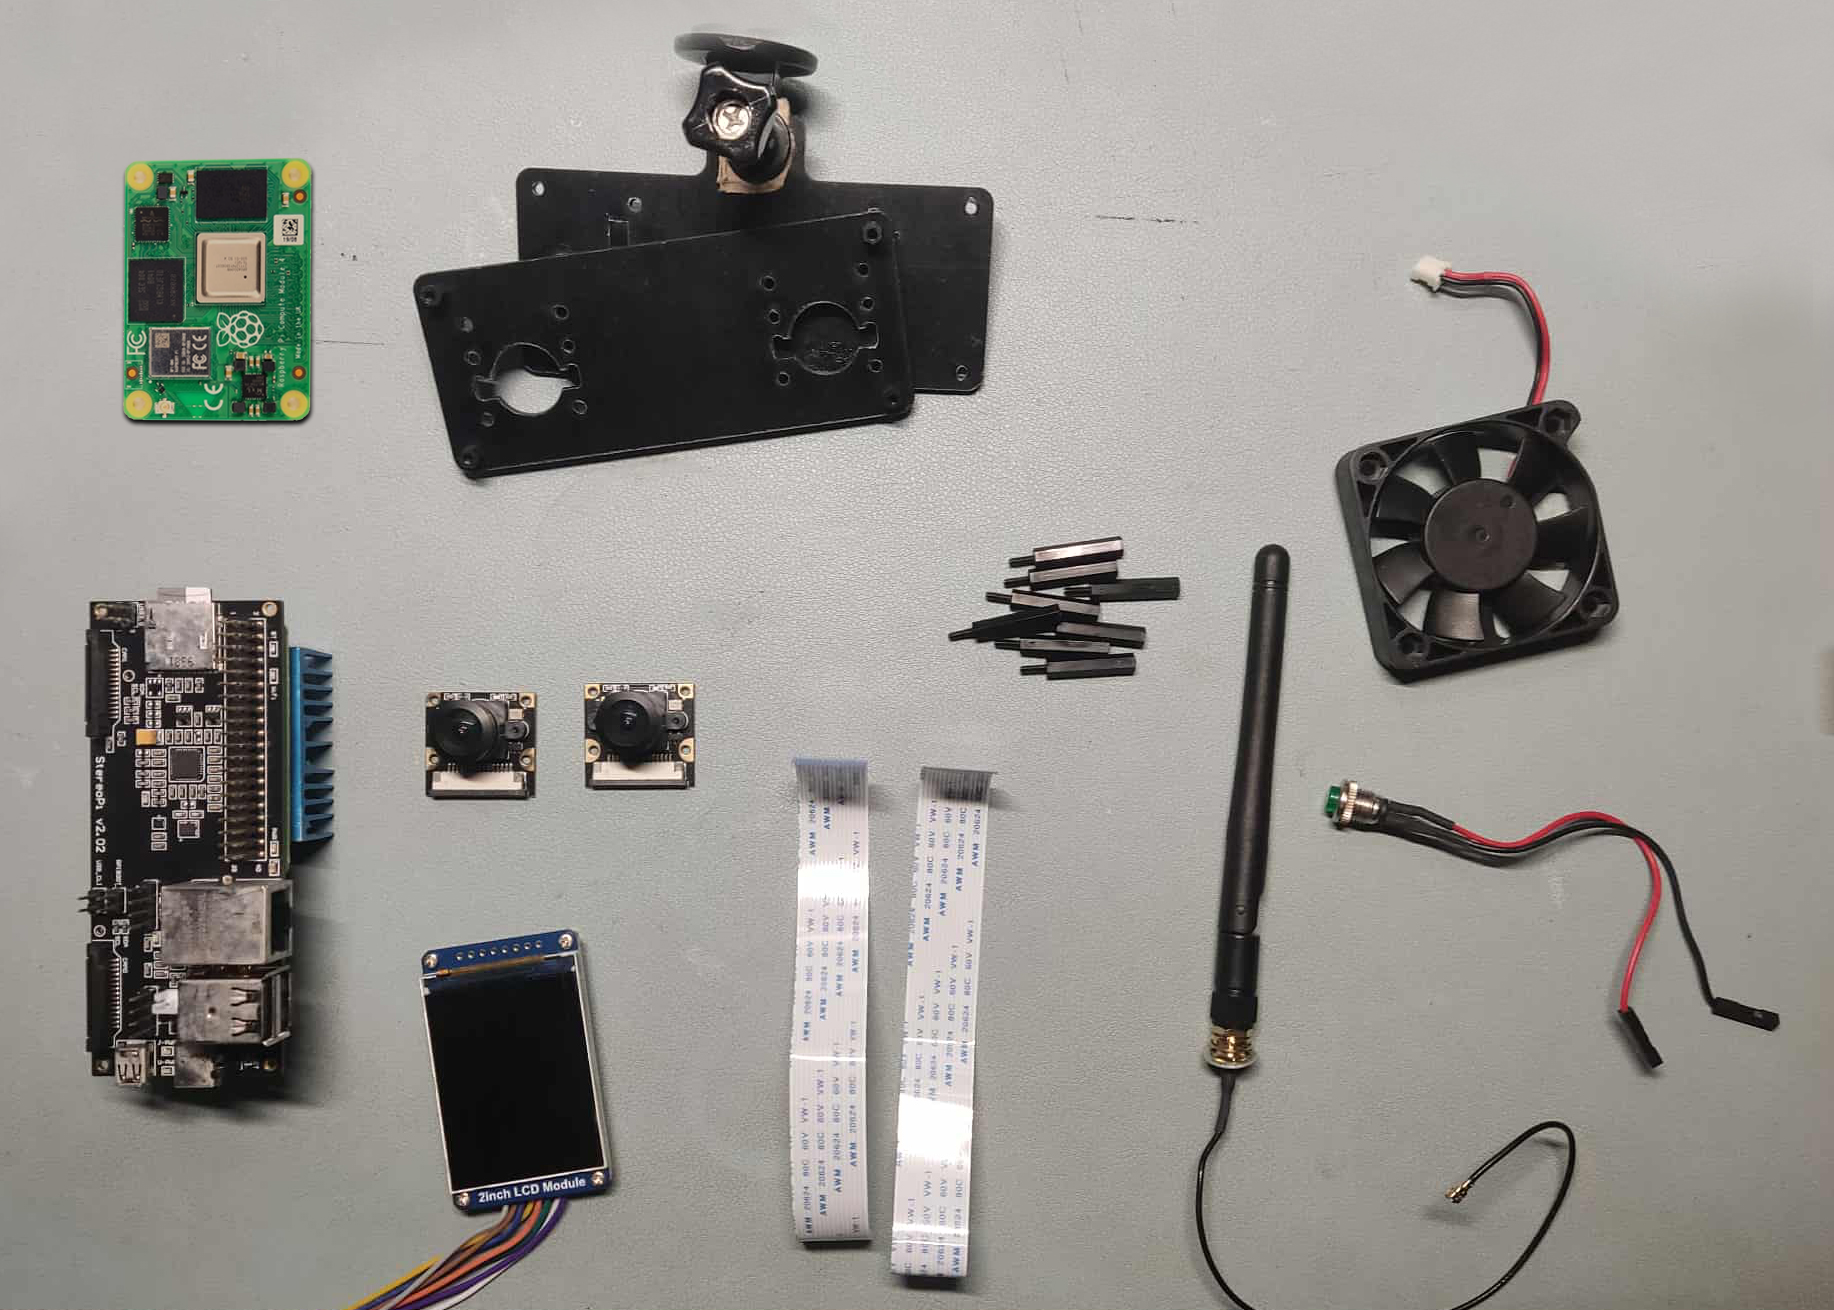
\includegraphics[width=\textwidth]{Parts.png}
	\captionof{figure}{Components used in the prototype development.From the top left: Raspberry Pi Computer Module 4, 3D Printed Custom Housing, cooling fan, StereoPi V2 Board, two camera modules, antenna,momentary push button, and 2-inch LCD module. }
\end{center}



\subsubsection{Prototype Building}
The prototype involved the StereoPi V2 Kit which was acquired through an official international distributer. After assembling the camera, it was further modified to address the it's heating by incorporating a heat sink and a small computer fan to make it suitable for outdoor use.


\begin{minipage}{0.45\textwidth}
	\centering
	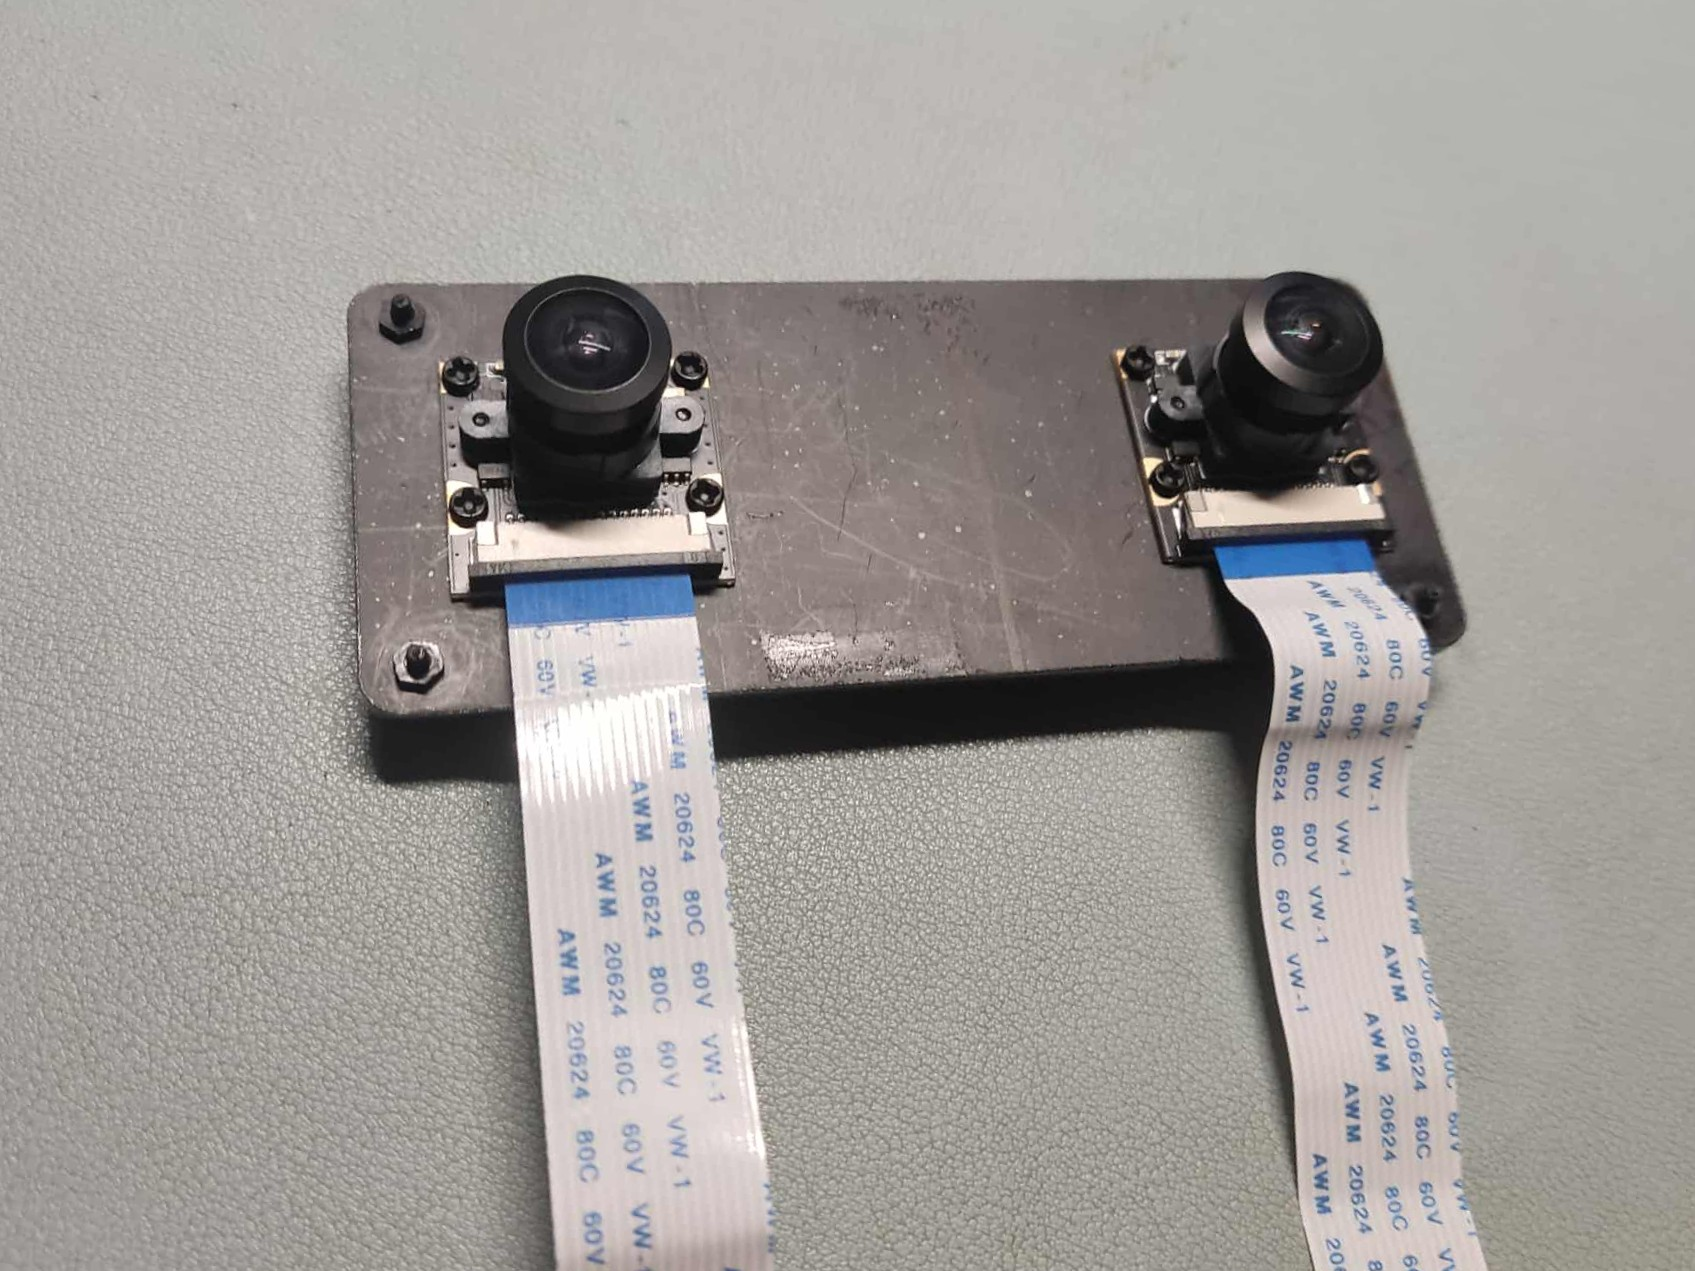
\includegraphics[width=\textwidth]{3.jpg}
	\captionof{figure}{Dual RPi Camera Modules attached to the custom housing.}
\end{minipage}
\hfill
\begin{minipage}{0.45\textwidth}
	\centering
	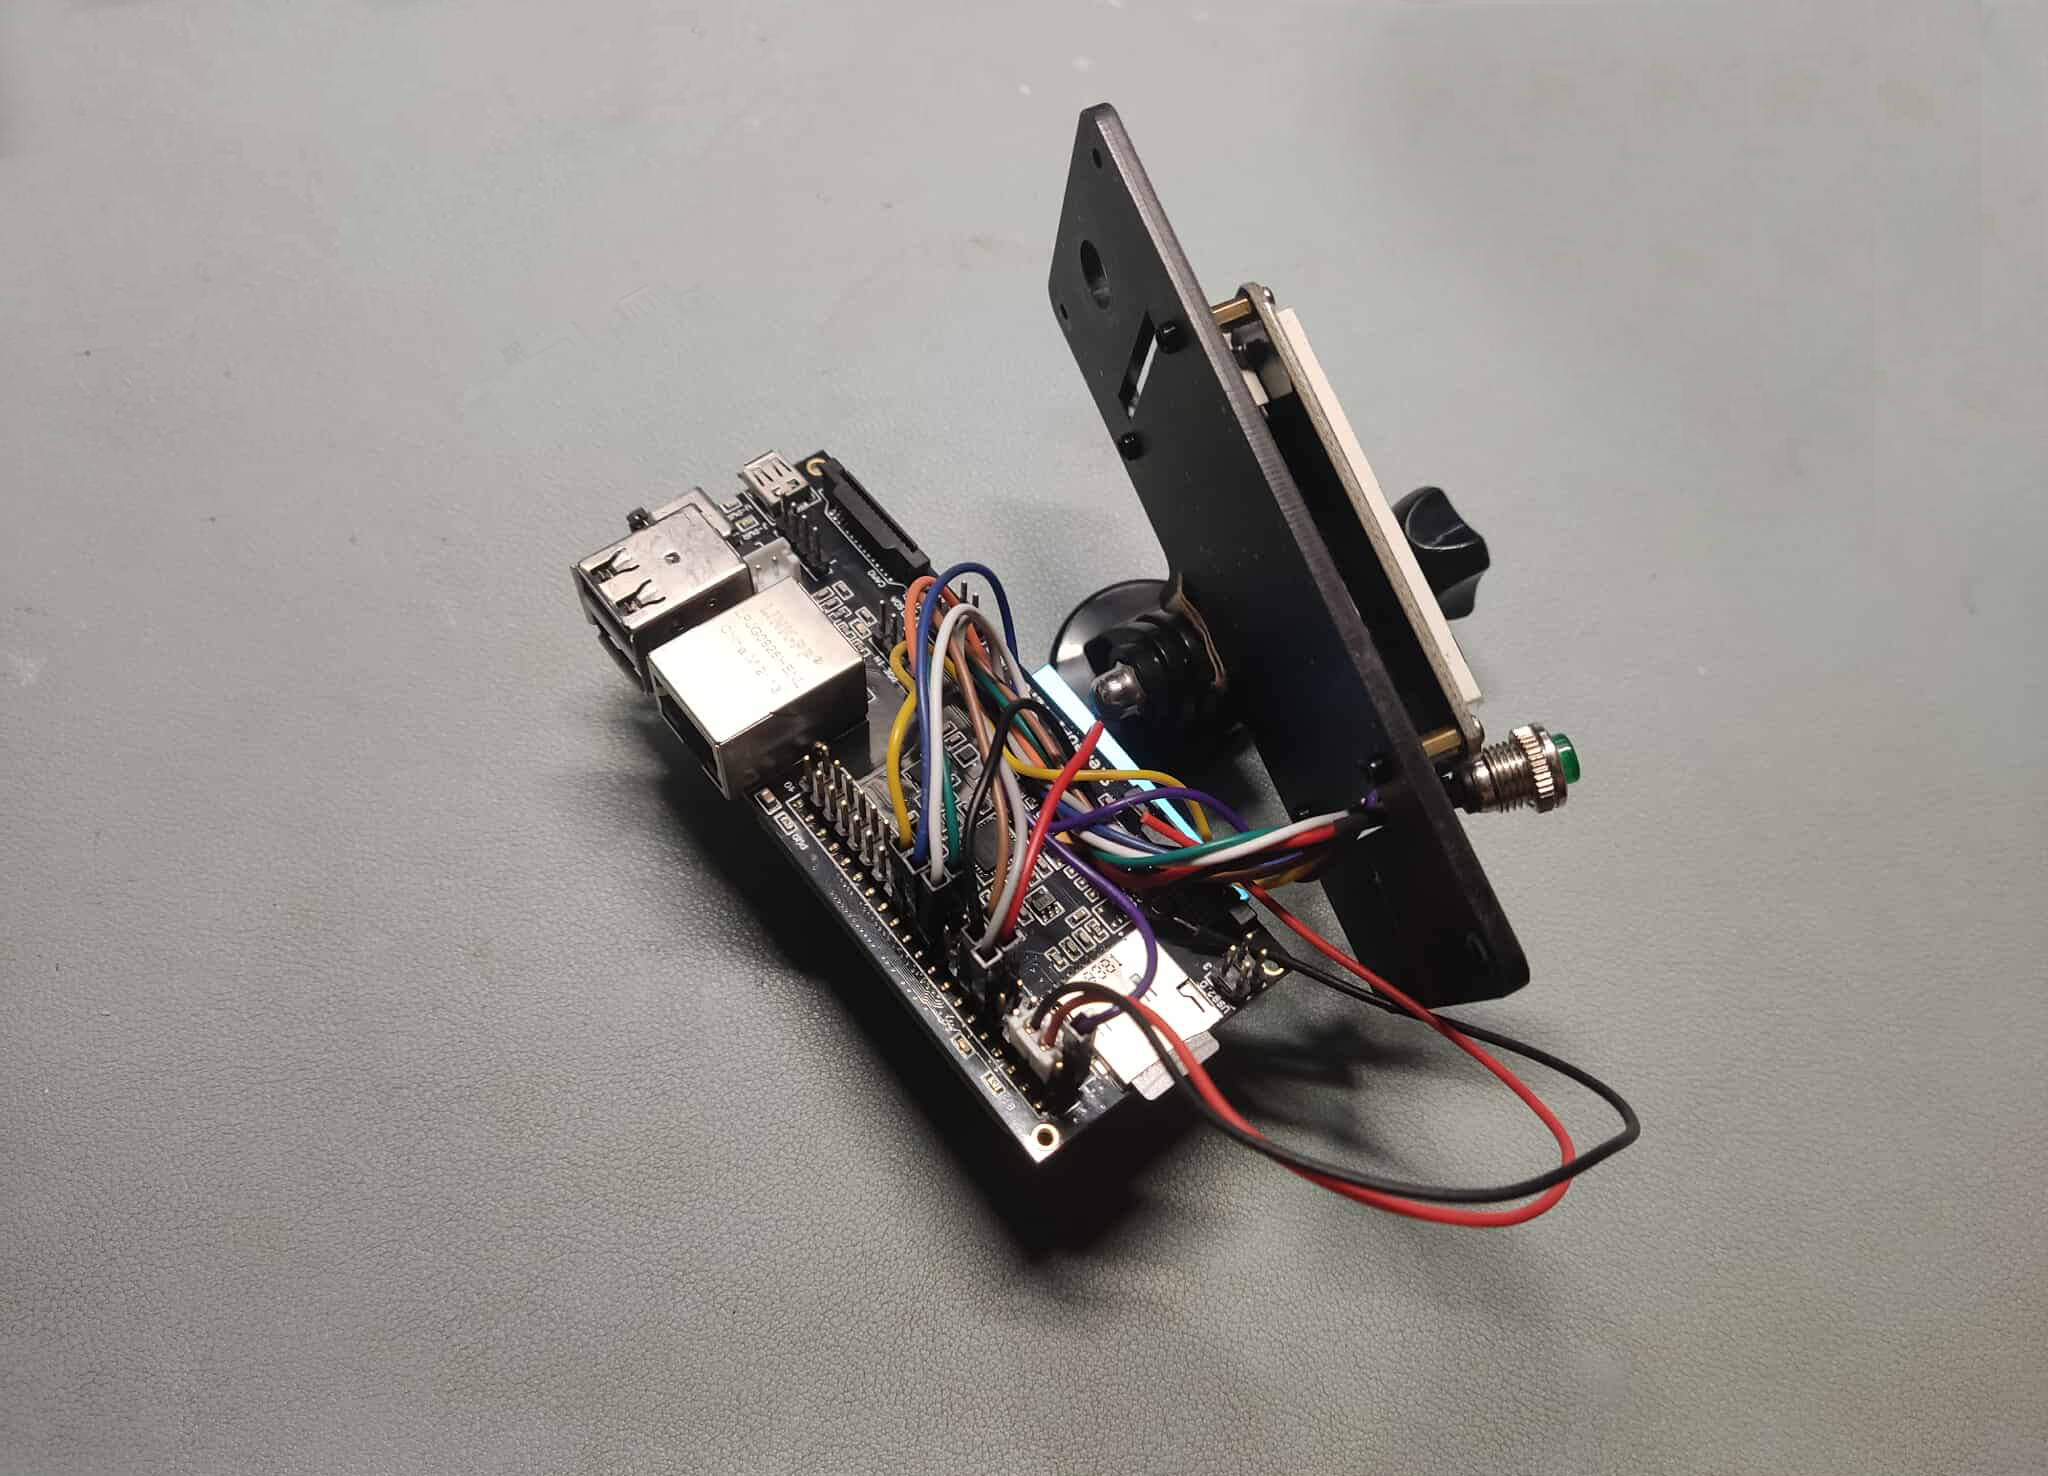
\includegraphics[width=\textwidth]{1.jpg}
	\captionof{figure}{LCD Module connected to the StereoPi board.}
	\label{fig:pic2}
\end{minipage}

%Partial Build%
\begin{center}
	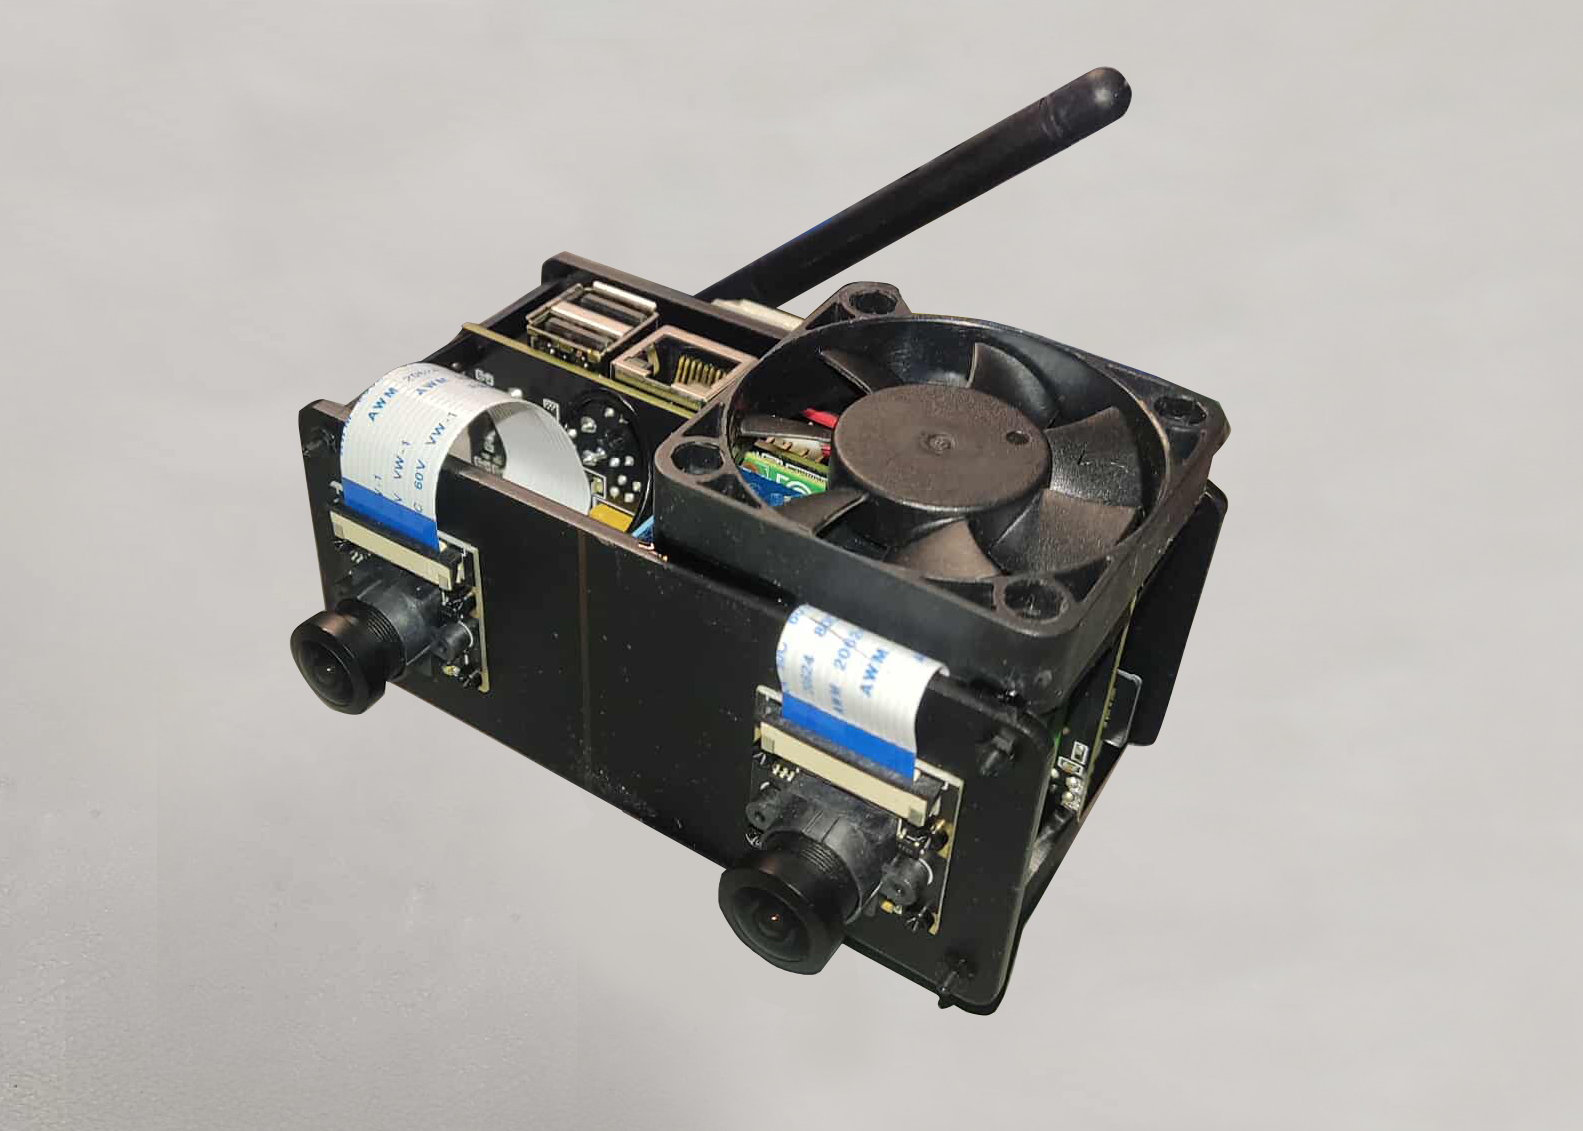
\includegraphics[scale=0.20]{prototype.png}
	\captionof{figure}{The finished prototype.}
\end{center}


\subsubsection{Camera Calibration (Fisheye Distortion)}
The StereoPi V2 is first calibrated using a 9 by 6 checkerboard, with a checker size of 55mm, from different angles through calibration scripts that came with the package. This process ensured that the camera is working properly in capturing stereo imagery. This removed distortion from captured images allowing depth estimation with more accuracy. 

%calibration
\begin{center}
	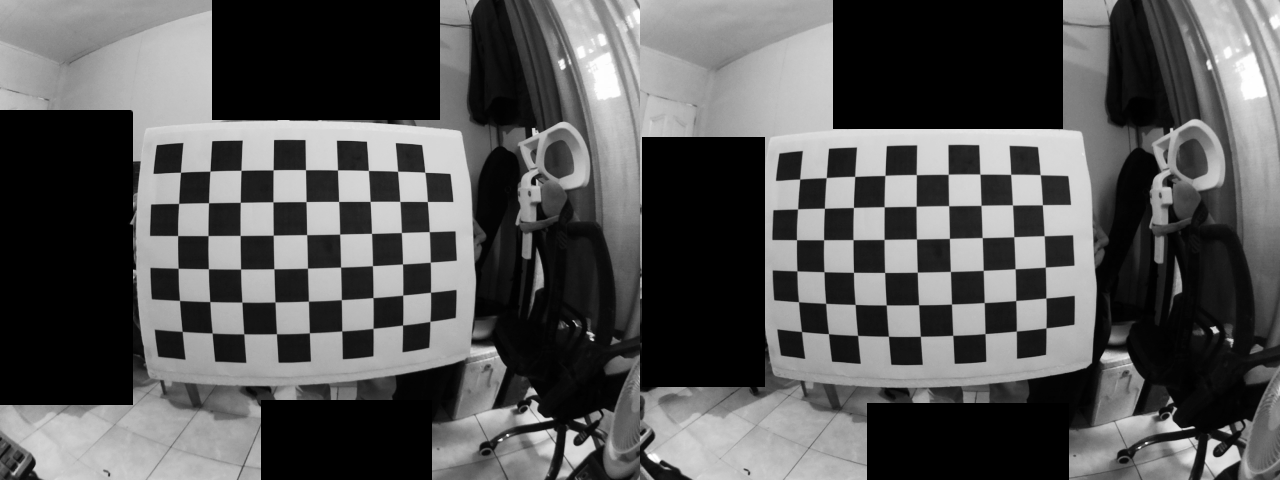
\includegraphics[scale=0.25]{calibration.png}
	\captionof{figure}{Calibration process with a checkerboard to correct fisheye lens distortion.}
\end{center}

\subsubsection{Camera Calibration (Disparity  Map Fine-tuning)}
The stereo image pairs captured by the system were first rectified to ensure proper alignment of corresponding features. Block matching parameters were then fine-tuned to produce clearer and more accurate disparity maps. It was observed that the effective operational range of the stereo camera system extends from approximately 30 to 80 cm. At distances closer than 30 cm, the disparity maps exhibited significant noise, while at distances beyond 80 cm, disparity information became sparse or blank.

%calibration2
\begin{center}
	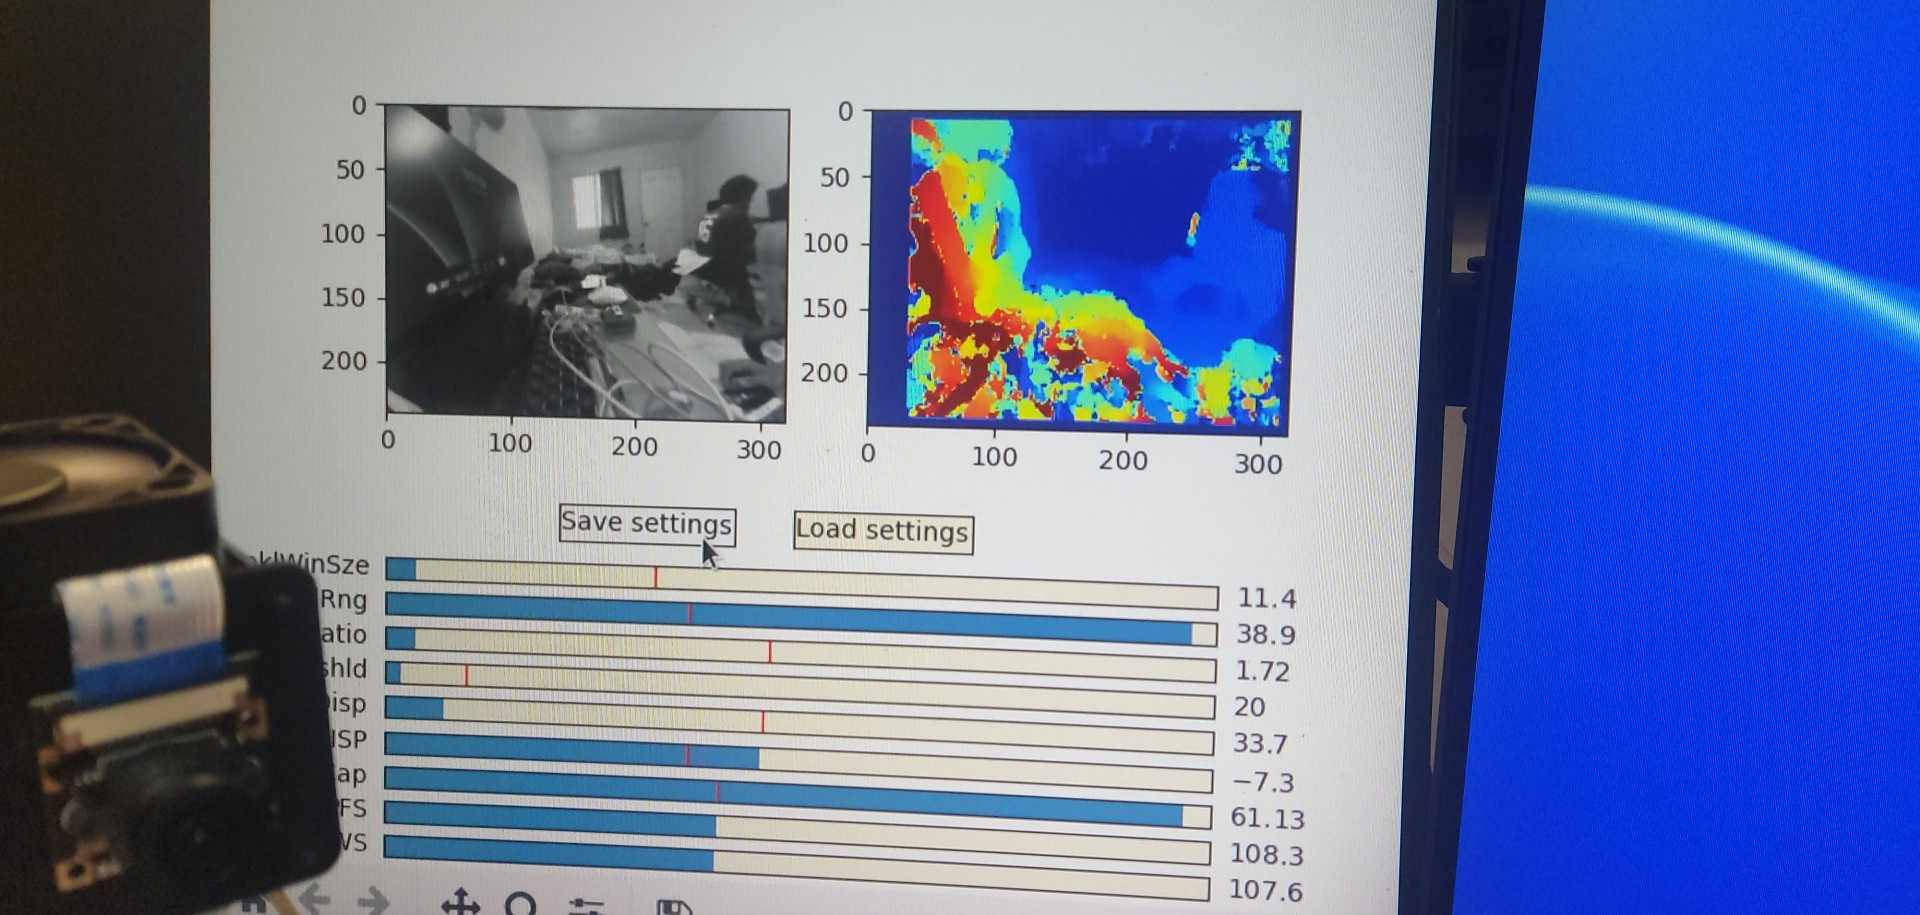
\includegraphics[scale=0.15]{calibration2.jpg}
	\captionof{figure}{Parameter tuning process to achieve cleaner and more accurate disparity maps.}
\end{center}

\subsubsection{Initial Testing}
Initial testing was conducted to verify the functionality and basic accuracy of the stereoscopic camera system in a controlled environment. Artificial potholes with known depths were created to simulate varying real-world scenarios. The system captured disparity maps, and estimated depths were computed using the standard stereo camera depth formula.

%initial test
\begin{center}
	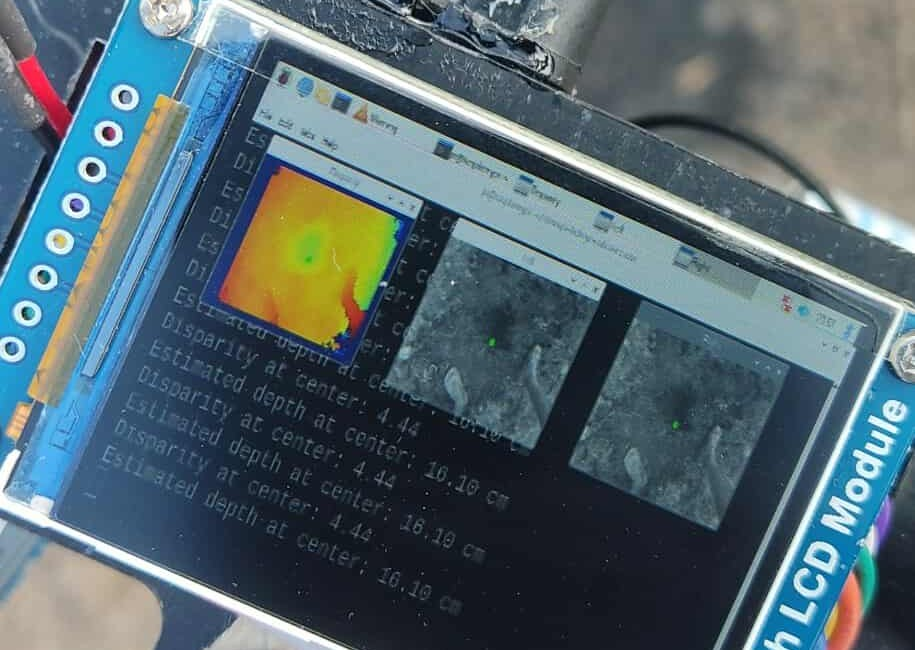
\includegraphics[scale=0.35]{initialtest.jpg}
	\captionof{figure}{The system tested on a simulated pothole.}
\end{center}

However, the results revealed a non-linear relationship between the computed disparity values and the actual distances. This discrepancy indicated that the traditional depth estimation method was insufficient for the current setup. To address this, the researchers collected multiple data points and correlating known distances to their respective disparity readings and fitted an inverse model to better represent the system's behavior (see Figure 3.10). This updated disparity-to-depth model was subsequently used in the final testing phase.

%initial test
\begin{figure}[H]
	\centering
	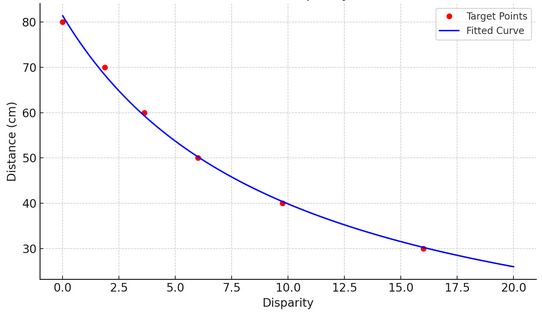
\includegraphics[scale=0.55]{inversemodel.png}
	\caption{Inverse Model Fit to Disparity vs. Distance.\\}
	\label{fig:inverse}
\end{figure}




\subsubsection{Performance Metrics}
The accuracy of the pothole depth estimated by StereoPi V2 was analyzed using Linear Regression in order to model the difference between the disparity and distance. The lower the disparity indicates that the pothole is deeper.

%The performance of the YOLOv5 model will be evaluated using mean Average Precision (mAP). mAP is a widely used metric in object detection tasks and is particularly useful for assessing models that need to detect and classify multiple object categories. In this case, mAP will provide a comprehensive evaluation of the model's ability to detect and classify potholes, offering an aggregated score across the relevant detection thresholds. This ensures a balanced assessment of both detection accuracy and classification performance, which is essential for accurately identifying potholes across varying conditions. The effectiveness of mAP for this task is well-established in object detection literature (Everingham et al., 2015; Lin et al., 2014).



%For the accuracy of depth estimation using the Epipolar Spatio-Temporal Networks (ESTN), Root Mean Squared Error (RMSE) and Mean Absolute Error (MAE) will be used. RMSE is chosen for its ability to penalize larger errors more heavily, making it suitable for assessing depth estimation performance where larger deviations from the ground truth are more significant (Zhang et al., 2018). MAE is also employed to provide a straightforward measure of average error magnitude, offering a complementary evaluation of depth estimation without emphasizing larger errors as much (Zhang et al., 2020).

\subsubsection{Final Testing and Validation}
The testing process began with a detailed testing plan that includes both simulated and real-world testing scenarios. Initially, the system is tested in controlled environments to verify its capability to estimate pothole depth effectively. Following this, real-world testing was conducted using the StereoPi kit on previously located potholes, specifically at the University of the Philippines Visayas Miagao Campus. The procedure for estimating pothole depth closely followed the validated depth measurement manual where the system captured depth measurements at four designated points within each pothole, corresponding to the measure points used in the manual measurement data. These four estimated depths were then averaged to determine the final depth estimate for each pothole. The system's performance was validated by comparing its predictions with ground-truth data collected from manual inspections. 

\begin{figure}[H]
	\centering
	\begin{minipage}{0.45\textwidth}
		\centering
		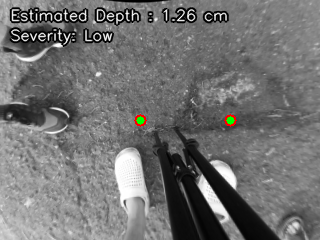
\includegraphics[width=\textwidth]{measure1.png}
		\caption{First measure point}
		\label{fig:image1}
	\end{minipage}
	\hfill
	\begin{minipage}{0.45\textwidth}
		\centering
		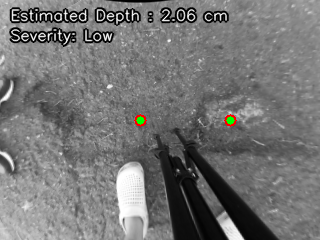
\includegraphics[width=\textwidth]{measure2.png}
		\caption{Second measure point}
		\label{fig:image2}
	\end{minipage}
\end{figure}
%	\vskip\baselineskip
\begin{figure}[H]
	\begin{minipage}{0.45\textwidth}
		\centering
		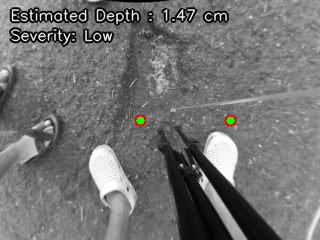
\includegraphics[width=\textwidth]{measure3.png}
		\caption{Third measure point}
		\label{fig:image3}
	\end{minipage}
	\hfill
	\begin{minipage}{0.45\textwidth}
		\centering
		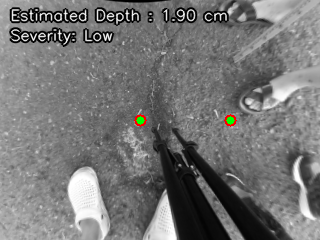
\includegraphics[width=\textwidth]{measure4.png}
		\caption{Fourth measure point}
		\label{fig:image4}
	\end{minipage}
\end{figure}


\subsubsection{Documentation}
Throughout the research activities, thorough documentation was maintained. This documentation captured all methods, results, challenges, and adjustments made during the experimentation phases. It ensured the reproducibility of the work and provided transparency for future research endeavors. 

\subsection{Challenges and Limitations}

\subsubsection{Camera Limitations}
During the data collection process, the researchers were faced with various issues involving the StereoPi V2 kit. Issues like inaccuracies in the rectified image pair and generated disparity map were very apparent in the early stages of data collection due to limited related studies and literature involving the camera. In addition, the camera also yielded some inaccurate depth estimation and over reliance on controlled environments which prompted the researchers to further improve its tuning and calibration. It was also observed that the effective working range of the camera for accurate depth estimation was limited to a distance of approximately 30cm to 80cm from the subject. Measurements taken outside of this range tended to result in noisy disparity maps or failed to distinguish objects properly in the disparity output, leading to unreliable depth values.

%\subsubsection{Availability of Local Datasets}
%The lack of locally labeled datasets for road defects has posed a challenge in training accurate models. The majority of available datasets are sourced from international locations, which may not fully represent the road conditions found in the study area. To address the lack of locally labeled datasets, the researchers will create a pilot dataset from local roads within the University of the Philippines Visayas Miagao Campus. This dataset will be manually annotated according to DPWH's classification standards, ensuring local relevance.

%\subsubsection{Data Quality and Variability}
%Variations in the quality and resolution of the data collected from different sources may impact the performance of the trained models. In particular, images captured under varying weather conditions or lighting may affect the accuracy of pothole detection. To address this, the researchers plan to use the StereoPi kit to capture images under optimal weather and lighting conditions, such as mid-morning or early afternoon on clear days, ensuring consistent image quality for stereo vision analysis. The kit’s stereo cameras will be calibrated for uniform resolution and focus. Data augmentation techniques will also be applied to simulate varying conditions, and pre-processing steps like noise reduction and contrast enhancement will be used to improve the quality of the captured data. This approach aims to minimize the impact of environmental factors on the accuracy of road pothole detection and depth estimation.


%\section{Calendar of Activities}
%Table 1 shows a Gantt chart of the activities. Each bullet represents approximately one week's worth of activity.
%
%  the following commands will be used for filling up the bullets in the Gantt chart
%
%\newcommand{\weekone}{\textbullet}
%\newcommand{\weektwo}{\textbullet \textbullet}
%\newcommand{\weekthree}{\textbullet \textbullet \textbullet}
%\newcommand{\weekfour}{\textbullet \textbullet \textbullet \textbullet}

%
%  alternative to bullet is a star 
%
%\begin{comment}
%\newcommand{\weekone}{$\star$}
% \newcommand{\weektwo}{$\star \star$}
% \newcommand{\weekthree}{$\star \star \star$}
% \newcommand{\weekfour}{$\star \star \star \star$ }
%\end{comment}



%\begin{table}[ht]   %t means place on top, replace with b if you want to place at the bottom
%\centering
%\caption{Timetable of Activities for 2024} \vspace{0.25em}
%\begin{tabular}{|p{2in}|c|c|c|c|c|} \hline
%\centering Activities (2024) & Aug   & Sept & Oct & Nov & Dec  \\ \hline
%Pre-proposal Preparation      &  \weekfour     &     &  &  &   \\ \hline
%Literature Review & ~~~\weekthree  & \weekone  & &  &    \\ \hline
%Data Collection     &  \weektwo & \weektwo  &  &  &  \\ \hline
%Algorithm Selection     &   & \weektwo &  &  &  \\ \hline
%System Design      &   & \weekone  & \weektwo & ~~~\weektwo &    \\ \hline
%Preliminary Testing &   &  &  & \weektwo & \weekone  \\ \hline
%Documentation and SP Writing & ~~~\weekfour & \weekfour & \weekfour & \weekfour & \weektwo \\ \hline
%\end{tabular}
%\label{tab:timetableactivities}
%\end{table}

%\begin{table}[ht]   %t means place on top, replace with b if you want to place at the bottom
%	\centering
%	\caption{Timetable of Activities for 2025} \vspace{0.25em}
%	\begin{tabular}{|p{2in}|c|c|c|c|c|c|} \hline
	%		\centering Activities (2025) & Jan   & Feb & Mar & Apr & May & Jun  \\ \hline
	%		Data Collection      &  \weekfour     &     &  &  & &  \\ \hline
	%		System Design & ~~~\weekthree  & \weektwo  & \weektwo &  & &   \\ \hline
	%		Model testing     &  \weekthree & \weekfour  &  \weekfour &  &  & \\ \hline
	%		Results Analysis    &   &  &  \weektwo & \weekfour& & \\ \hline
	%		Conclusion Formulation     &   &   &  & ~~~\weektwo &  ~~~\weekthree &  \\ \hline
	%		Documentation and SP Writing & ~~~\weekfour & \weekfour & \weekfour & \weekfour & \weekfour &% \weektwo\\ \hline
	%	\end{tabular}
%	\label{tab:timetableactivities}
%\end{table}


               %LaTeX source file for Chapter 3: Methodology
%   Filename    : chapter_4.tex 
\chapter{Preliminary Results/System Prototype}
This chapter presents the results on estimating the depth of potholes using the StereoPi system. It details the prototype construction, calibration of the system, and the application of regression analysis to improve depth estimation. It also contains the measurements taken during the testing phases, comparing the ground truth depths with the value estimated by the camera. Findings are presented systematically, supported by tables showing the collected data, images of the outputs, and discussion on the analysis of results.

\section{\textbf{System Calibration and Model Refinement}}
After the initial testing, the system was calibrated using a controlled setup, where artificial potholes with known depths were created. The stereo camera system captured disparity maps, from which depth was calculated using the standard stereo vision formula:

\[
\text{Depth} = \frac{f \times B}{d}
\]

where:
\begin{itemize}
	\item \( f \) is the focal length in pixels,
	\item \( B \) is the baseline distance between the two cameras,
	\item \( d \) is the disparity.
\end{itemize}


However, preliminary observations revealed that the relationship between measured disparity and true depth was nonlinear, particularly for small disparities corresponding to greater distances. As a result, a direct application of the stereo formula led to systematic errors, especially at the extremes of the depth range.

To address the nonlinear behavior, a curve fitting approach was introduced. Specifically, an inverse model was fitted to the collected data points, relating disparity and ground-truth distance measurements.

An inverse function of the form:

\[
y = a + \frac{b}{x}
\]

where:
\begin{itemize}
	\item \( y \) is the estimated distance (in cm),
	\item \( x \) is the measured disparity,
	\item \( a \) and \( b \) are coefficients obtained through regression analysis.
\end{itemize}

\section{\textbf{Model Refinement Using Regression}}
The regression analysis produced the following model parameters:
\begin{itemize}
	\item a = …
	\item b = ...
\end{itemize}

The model achieved the following performance on the test data:

\begin{table}[H]
	\centering
	\begin{tabular}{|c|c|}
		\hline
		\textbf{Metric} & \textbf{Value} \\ \hline
		Mean Absolute Error (MAE) & X cm \\ \hline
		Root Mean Square Error (RMSE) & X cm \\ \hline
	\end{tabular}
	\caption{Performance Metrics for the Regression Model}
	\label{tab:performance_metrics}
\end{table}

The relatively low MAE and RMSE indicate that the fitted model significantly improved the accuracy of depth estimation compared to the original stereo formula.


\section{\textbf{Error Analysis}}
Despite the improvements, minor estimation errors remained. These errors were primarily attributed to:
\begin{itemize}
	\item Low-light imaging conditions affecting disparity computation,
	\item Shallow potholes with depths less than 3 cm, where disparity resolution becomes a limiting factor,
	\item Perspective distortion when the stereo camera was not parallel to the ground plane.
\end{itemize}


\section{\textbf{Testing Results} }
Following calibration, actual potholes located around the University of the Philippines Visayas (UPV) campus were tested. The ground truth depths of the potholes were measured manually and compared with the depths estimated by the camera. Based on the results, the StereoPi camera was able to estimate the depths fairly close to the ground truth values.The smallest difference was seen in Pothole 5, where the estimated depth was only 0.24 cm away from the ground truth. The largest difference was found in Pothole 1, where the error was 3.45 cm. For the other potholes, the differences were 0.67 cm for Pothole 2, 2.07 cm for Pothole 3, and 2.66 cm for Pothole 4. Most of the time, the camera’s estimated depths were only off by about one to three centimeters. Table \ref{tab:comparison} shows the comparison between the manually measured ground truth depths and the depths estimated by the StereoPi camera for each simulated pothole.

\begin{table}[H]
	\centering
	\hspace{-2cm}
	\small 
	\caption{Ground Truth and StereoPi Depth Measurements}
	\begin{tabular}{|p{1.5cm}|p{1.5cm}|p{1.5cm}|p{1.5cm}|p{1.5cm}|p{1.5cm}|p{1.5cm}|p{1.5cm}|}
		\hline
		\textbf{Pothole} & \textbf{Ground Truth 1 (cm)} & \textbf{Ground Truth 2 (cm)} & \textbf{Ground Truth Avg (cm)} & \textbf{Est Depth 1(cm)} & \textbf{Est Depth 2 (cm)} & \textbf{Est Depth Avg(cm)} & \textbf{Diff(cm)} \\ \hline
		
		1 & 14.6 & 14.4 & 14.5 & 11.16 & 10.94 & 11.05 & 3.45  \\ \hline
		2 & 12.0 & 12.1 & 12.05 & 12.36 & 10.4 & 11.38 & 0.67 \\ \hline
		3 & 6.4 & 6.5 & 6.45 & 4.76 & 4.0 & 4.38 & 2.07 \\ \hline
		4 & 9.8 & 9.3 & 9.55 & 6.16 & 7.62 & 6.89 & 2.66 \\ \hline
		5 & 13.9 & 14.3 & 14.1 & 13.04 & 14.68 & 13.86 & 0.24 \\ \hline
		
	\end{tabular}
	\label{tab:comparison}
	\hspace{-3cm}
\end{table}

\begin{figure}[htbp]
	\centering
	\begin{minipage}{0.32\textwidth}
		\centering
		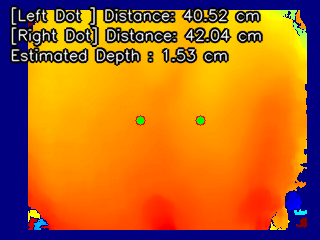
\includegraphics[width=\textwidth]{disparity.png}
		\caption{Disparity Map}
		\label{fig:image1}
	\end{minipage}
	\hfill
	\begin{minipage}{0.32\textwidth}
		\centering
		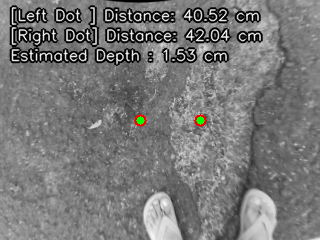
\includegraphics[width=\textwidth]{left.png}
		\caption{Left Stereo Image}
		\label{fig:image2}
	\end{minipage}
	\hfill
	\begin{minipage}{0.32\textwidth}
		\centering
		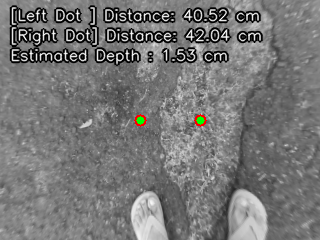
\includegraphics[width=\textwidth]{right.png}
		\caption{Right Stereo Image}
		\label{fig:image3}
	\end{minipage}
\end{figure}



\section{\textbf{Discussion}}

     
\chapter{Conclusion}
This chapter provides conclusions based on the research findings from data collected on the development of a pothole depth estimation system using stereo vision technology.It then presents recommendations for practice and suggestions for further research.

\section{Summary}
This special project addressed the critical issue of road maintenance by developing a system capable of estimating the depth of potholes to help prioritize repairs. The purpose of the project was to create an automated method that not only detects potholes but also assesses their severity based on depth, responding to the current manual and slow road inspection practices. The researchers aimed to collect high-quality images of potholes under varying conditions, to validate the system’s depth estimation accuracy using ground truth measurements and linear regression analysis, and to build a working prototype using stereo vision that can detect, measure, and assess potholes. 

To achieve these objectives, a hardware prototype was built using the StereoPi V2 board and Raspberry Pi Compute Module 4, equipped with dual fisheye-lens cameras. Camera calibration was performed using a 9x6 checkerboard pattern with known square sizes to correct for fisheye lens distortion and ensure proper alignment of the stereo pair. After calibration, disparity map generation was fine-tuned by adjusting block matching parameters to produce clearer and more reliable disparity maps. Initial testing was conducted using simulated potholes with known depths to verify the functionality of the system and identify the non-linear behavior present in stereo vision depth measurements. It was observed that using the standard stereo depth formula led to inaccuracies, particularly at greater distances. 

The calibrated system and fitted regression model were validated by comparing the estimated depths with the manually measured depths. The findings showed that the system was able to estimate pothole depths within approximately ±3 cm of actual measurements, achieving a Mean Absolute Error (MAE) of 0.945 cm and a Root Mean Square Error (RMSE) of 0.844 cm. A strong positive linear relationship was observed between the estimated and actual depths (R = 0.978, R² = 0.956).

\section{Conclusions}
The researchers conclude the following based on the findings:

\begin{itemize}
	\item The system effectively captures and analyzes depth information from stereo images, providing a viable method for automated pothole severity assessment.
	
	\item Incorporating depth measurements significantly improves pothole repair prioritization compared to traditional visual-only inspections, allowing maintenance decisions to be based on objective, measurable data.
	\item The system achieved an acceptable regression model fit, with a strong positive correlation (R = 0.978) and a coefficient of determination (R² = 0.956), confirming that the depth estimates closely align with the ground truth measurements.The system obtained satisfactory error metrics, with a Mean Absolute Error (MAE) of 0.945 cm and a Root Mean Square Error (RMSE) of 0.844 cm, indicating reliable performance for both pothole detection and depth estimation tasks.
	\item The proposed approach fills a critical gap in current road maintenance practices, especially within the Philippine context where depth-based severity classification is not yet systematically implemented.
\end{itemize}

This special project has successfully developed a system that addresses the problem of pothole severity assessment using depth measurement.The research shows that stereo vision, even using accessible and affordable technology, holds strong potential for future development in road maintenance automation. By building upon the foundation laid by this project, future systems can become even more accurate, efficient, and practical for real-world deployment

\section{Recommendations for Practice}
Based on the findings of this special project, the following recommendations are proposed for future researchers, engineers, and road maintenance agencies:

\textit{Use stereo vision systems for road surveys.} In contexts where LiDAR-based technologies may be cost-prohibitive, maintenance agencies should consider adopting calibrated stereo vision systems for estimating pothole depth. This approach offers a more cost-effective alternative while still enabling depth-based severity classification, thereby allowing for more objective and data-driven prioritization of road repairs compared to traditional visual inspections.

\textit{Incorporate depth-based severity classification in maintenance procedures}. Authorities should update road inspection protocols to include depth measurements, making pothole severity assessment more objective and standardized.


\section{Suggestions for further research}

Based on the limitations encountered and the results obtained,the researchers have
observed that there are lapses and possible improvements to further better this system.

\textit{Better camera}. While the StereoPi V2 camera was effective for basic depth estimation, its performance is limited by its resolution, sensitivity to lighting, and depth range. Future researchers could consider using higher-quality stereo cameras or depth sensors with better image resolution and low-light capabilities to achieve more accurate and consistent disparity maps.
	
\textit{Improve camera calibration and tuning}. While the StereoPi system produced good depth estimates, the results still varied depending on the precision of the camera calibration. Future researchers can explore better calibration techniques and finer parameter adjustments to minimize errors, especially in challenging environments.

\textit{Use of multi-camera arrays.} Instead of relying solely on a two-camera stereo setup, future research could explore the use of multi-point or multi-angle camera arrays. These systems can offer improved depth perception and coverage, particularly for complex or uneven road surfaces, by capturing more comprehensive 3D data.

\textit{Integration of stereo vision with motion-based analysis.} Incorporating frame differencing techniques, similar to motion detection algorithms, could be beneficial for dynamic environments or mobile applications. This approach may simulate the effect of a moving vehicle and allow the system to detect and estimate potholes more robustly in real time, enhancing its applicability for onboard vehicle-mounted systems.          %LaTeX source file for Chapter 4: Preliminary Results/System Prototype

%\bibliographystyle{apacite}       %-- specified APA style for bibliograpy
% www.ctan.org/tex-archive/biblio/bibtex/contrib/apacite/
%-- bibliographic entries are handled via bibtex; refer to www.bibtex.org for more details
\bibliography{references}       %-- the file "myreferences.bib" is a sample bibliography 

\appendix                         %specify appendices
%%%%%%%%%%%%%%%%%%%%%%%%%%%%%%%%%%%%%%%%%%%%%%%%%%%%%%%%%%%%%%%%%%%%%%%%%%%%%%%%%%%%%%%%%%%%%%%%%%%%%%
%
%   Filename    : appendix_A.tex 
%
%   Description : This file is for including the Research Ethics Documents (delegated as Appendix A) 
%                 
%%%%%%%%%%%%%%%%%%%%%%%%%%%%%%%%%%%%%%%%%%%%%%%%%%%%%%%%%%%%%%%%%%%%%%%%%%%%%%%%%%%%%%%%%%%%%%%%%%%%%%

\chapter{Code Snippets}
\label{sec:appendixa}

\begin{lstlisting}[language=Python, caption={Function for generating stereo depth map and classifying pothole severity based on depth difference between two points}]
	def stereo_depth_map(rectified_pair, save_path_prefix=None):
	global disp_max, disp_min
	dmLeft, dmRight = rectified_pair
	
	disparity_raw = sbm.compute(dmLeft, dmRight).astype(np.float32)
	disparity_raw /= 16.0  # normalize disparity
	
	local_max, local_min = disparity_raw.max(), disparity_raw.min()
	
	if dm_colors_autotune:
	disp_max = max(local_max, disp_max)
	disp_min = min(local_min, disp_min)
	local_max, local_min = disp_max, disp_min
	
	# Normalize for visualization
	disparity_vis = (disparity_raw - local_min) * (255.0 / (local_max - local_min))
	disparity_vis = np.uint8(np.clip(disparity_vis, 0, 255))
	disparity_color = cv2.applyColorMap(disparity_vis, cv2.COLORMAP_JET)
	
	# Calculate depth
	depth_map = calculate_depth(disparity_raw)
	
	# Define two points
	center_y, center_x = depth_map.shape[0] // 2, depth_map.shape[1] // 2 - 20
	second_y = center_y
	second_x = center_x + offset_x
	
	# Read depth and disparity values
	center_depth_cm = (depth_map[center_y, center_x]) 
	second_depth_cm = (depth_map[second_y, second_x]) 
	estimated_depth_cm = abs(center_depth_cm - second_depth_cm)
	
	# Define severity based on estimated depth
	if estimated_depth_cm < 2.5:
	severity = "Low"
	elif estimated_depth_cm >= 2.5 and estimated_depth_cm < 5.0:
	severity = "Medium"
	elif estimated_depth_cm > 5.0:
	severity = "High"
	else:
	severity = "Unknown"
\end{lstlisting}

\begin{lstlisting}[language=Python, caption={Main loop for capturing stereo image pairs, remapping them for rectification,and estimating depth}]
	for frame in camera.capture_continuous(capture, format="bgra", use_video_port=True, resize=(img_width,img_height)):
	pair_img = cv2.cvtColor(frame, cv2.COLOR_BGR2GRAY)
	
	imgLeft = pair_img[:, :img_width//2]
	imgRight = pair_img[:, img_width//2:]
	
	imgL = cv2.remap(imgLeft, leftMapX, leftMapY, interpolation=cv2.INTER_LINEAR, borderMode=cv2.BORDER_CONSTANT)
	imgR = cv2.remap(imgRight, rightMapX, rightMapY, interpolation=cv2.INTER_LINEAR, borderMode=cv2.BORDER_CONSTANT)
	
	if useStripe:
	imgL = imgL[80:160,:]
	imgR = imgR[80:160,:]
	
	stereo_depth_map((imgL, imgR), save_path_prefix=None)
	
	button_held_time = 0
	HOLD_THRESHOLD = 1.0  # seconds
	
	if GPIO.input(BUTTON_PIN) == GPIO.LOW:
	press_start = time.time()
	while GPIO.input(BUTTON_PIN) == GPIO.LOW:
	time.sleep(0.01)
	button_held_time = time.time() - press_start
	
	if button_held_time < HOLD_THRESHOLD:
	timestamp = datetime.now().strftime("%Y%m%d_%H%M%S")
	prefix = f"./captures/capture_{timestamp}"
	print(f"\n[!] Capturing snapshot at {timestamp}...")
	stereo_depth_map((imgL, imgR), save_path_prefix=prefix)
	time.sleep(0.5)
	else:
	cycle_offset()
	time.sleep(0.5)
\end{lstlisting}

% Save the file you want to include in PDF format.
% Uncomment the commant below specifying the correct appendix file. 
%\includepdf[pages=-, scale = 0.9, pagecommand={}, offset = -30 0]{appendixA.pdf}

              %LaTeX source file for Appendix A
%%%%%%%%%%%%%%%%%%%%%%%%%%%%%%%%%%%%%%%%%%%%%%%%%%%%%%%%%%%%%%%%%%%%%%%%%%%%%%%%%%%%%%%%%%%%%%%%%%%%%%
%
%   Filename    : appendix_B.tex
%
%   Description : This file will contain information about your Resource Persons
%                 
%%%%%%%%%%%%%%%%%%%%%%%%%%%%%%%%%%%%%%%%%%%%%%%%%%%%%%%%%%%%%%%%%%%%%%%%%%%%%%%%%%%%%%%%%%%%%%%%%%%%%%

\chapter{Resource Persons}
\label{sec:appendixb}

%
%  Indicate your resource persons here:
%
%	<full name and title, e.g., Dr. Juan de la Cruz>
%	<profession, e.g., faculty>
%	<department, e.g., Division of Physical Sciences and Mathematics>
%	<name of institution, e.g., University of the Philippines Visayas>
%	<e-mail address>
%
%

%
%  the following shows 3 examples, replace entries with your own
%

\newcommand{\resperson}[4]{\textbf{#1} \\ #2 \\ #3  \\ \url{#4}\vspace{0.5em}\\}

\resperson{Prof. Jumar Cadondon}{Assistant Professor}{Division of Physical Sciences and Mathematics} {University of the Philippines Visayas}{jgcadondon@up.edu.ph}

\resperson{Engr. Jane Chua}{Engineer}{DPWH Region 6}{chua.jane@dpwh.gov.ph}

\resperson{Engr. Marilou Zamora}{Chief}{Planning and Design}{DPWH Region 6}{zamora.marilou@dpwh.gov.ph}

\resperson{Engr. Benjamin Javellana}{Assistant Director}{Maintenance}{DPWH Region 6}{javellana.benjamin@dpwh.gov.ph}              %LaTeX source file for Appendix B
\chapter{Data Table and Stereo Pi Images}
\label{sec:appendixc}

\begin{table}[h!]
	\centering
	\resizebox{\textwidth}{!}{
		\begin{tabular}{|c|c|c|c|c|}
			\hline
			\textbf{Sample} & \textbf{Actual Depth (cm)} & \textbf{Estimated Depth (cm)} & \textbf{Residual} & \textbf{Absolute Error (cm)} \\
			\hline
			1 & 14.500 & 11.050 & -3.450 & 3.450 \\
			2 & 12.050 & 11.380 & -0.670 & 0.670 \\
			3 & 6.450 & 4.380 & -2.070 & 2.070 \\
			4 & 9.550 & 6.890 & -2.660 & 2.660 \\
			5 & 14.300 & 13.860 & -0.240 & 0.240 \\
			6 & 1.875 & 2.050 & 0.175 & 0.175 \\
			7 & 2.600 & 2.663 & 0.063 & 0.063 \\
			8 & 1.500 & 2.230 & 0.730 & 0.730 \\
			9 & 1.750 & 1.775 & 0.025 & 0.025 \\
			10 & 1.625 & 1.567 & -0.058 & 0.058 \\
			11 & 1.800 & 1.745 & -0.055 & 0.055 \\
			12 & 1.675 & 1.653 & -0.022 & 0.022 \\
			13 & 2.225 & 2.078 & -0.147 & 0.147 \\
			14 & 1.875 & 1.903 & 0.028 & 0.028 \\
			15 & 3.050 & 2.230 & -0.820 & 0.820 \\
			16 & 2.625 & 2.185 & -0.440 & 0.440 \\
			17 & 3.050 & 2.708 & -0.342 & 0.342 \\
			18 & 2.225 & 2.185 & -0.040 & 0.040 \\
			19 & 3.025 & 2.822 & -0.203 & 0.203 \\
			20 & 1.800 & 1.718 & -0.083 & 0.083 \\
			21 & 2.300 & 2.047 & -0.252 & 0.252 \\
			22 & 2.500 & 1.950 & -0.550 & 0.550 \\
			23 & 10.800 & 8.785 & -2.015 & 2.015 \\
			24 & 14.500 & 11.050 & -3.450 & 3.450 \\
			25 & 9.200 & 7.122 & -2.077 & 2.077 \\
			26 & 9.800 & 8.825 & -0.975 & 0.975 \\
			27 & 14.300 & 13.860 & -0.440 & 0.440 \\
			28 & 7.100 & 7.883 & 0.783 & 0.783 \\
			29 & 9.800 & 8.182 & -1.618 & 1.618 \\
			30 & 8.100 & 8.200 & 0.100 & 0.100 \\
			31 & 11.500 & 9.533 & -1.967 & 1.967 \\
			32 & 12.100 & 11.380 & -0.720 & 0.720 \\
			33 & 6.500 & 4.380 & -2.120 & 2.120 \\
			34 & 9.300 & 6.890 & -2.410 & 2.410 \\
			35 & 12.200 & 10.918 & -1.282 & 1.282 \\
			
			\hline
		\end{tabular}
	}
	\caption{Actual vs. Estimated Depths with Residuals and Absolute Errors}
	\label{tab:depth_results}
\end{table}

\begin{figure}[htbp]
	\centering
	\begin{minipage}{0.32\textwidth}
		\centering
		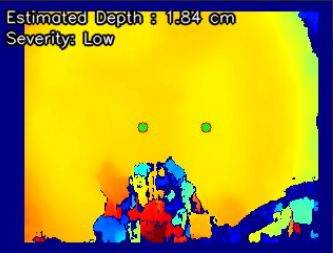
\includegraphics[width=\textwidth]{pothole disparity.png}
		\caption{Disparity Map}
		\label{fig:image1}
	\end{minipage}
	\hfill
	\begin{minipage}{0.32\textwidth}
		\centering
		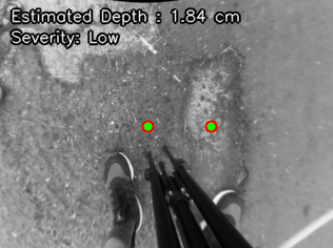
\includegraphics[width=\textwidth]{pothole raw left.png}
		\caption{Left Stereo Image}
		\label{fig:image2}
	\end{minipage}
	\hfill
	\begin{minipage}{0.32\textwidth}
		\centering
		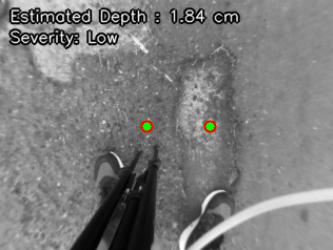
\includegraphics[width=\textwidth]{pothole raw right.png}
		\caption{Right Stereo Image}
		\label{fig:image3}
	\end{minipage}
\end{figure}              %LaTeX source file for Appendix C
\chapter{Supplementary Documents}
\label{sec:appendixd}

\begin{figure}[htbp]
	\centering
	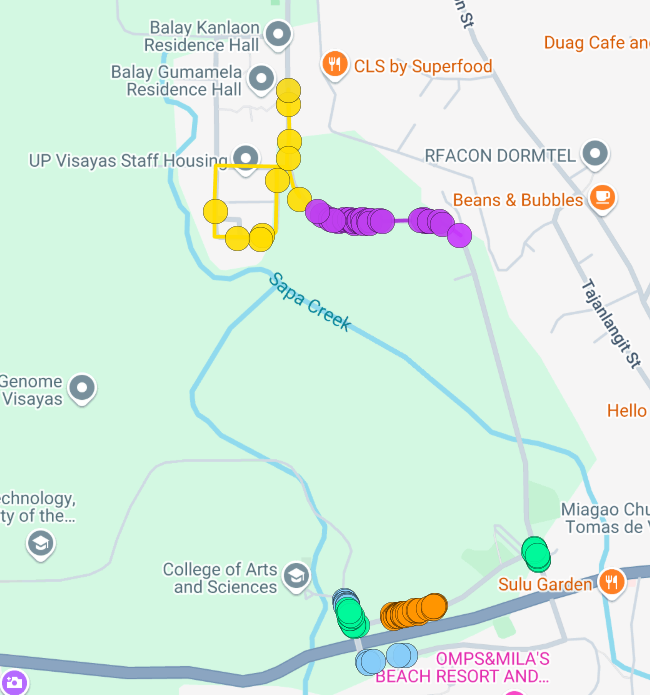
\includegraphics[height=10cm]{PHM_UPV.png}
	\caption{Visualized pothole locations during the ground truth data collection within the UPV campus.}
	\label{fig:pothole_map}
\end{figure}

\begin{figure}[htbp]
	\centering
	
\includegraphics[width=\textwidth]{DPWH_Letter.jpg}
	\caption{Letter requesting validation of data collection procedures.}
	\label{fig:validation_letter}
\end{figure}

\begin{figure}[htbp]
	\centering
	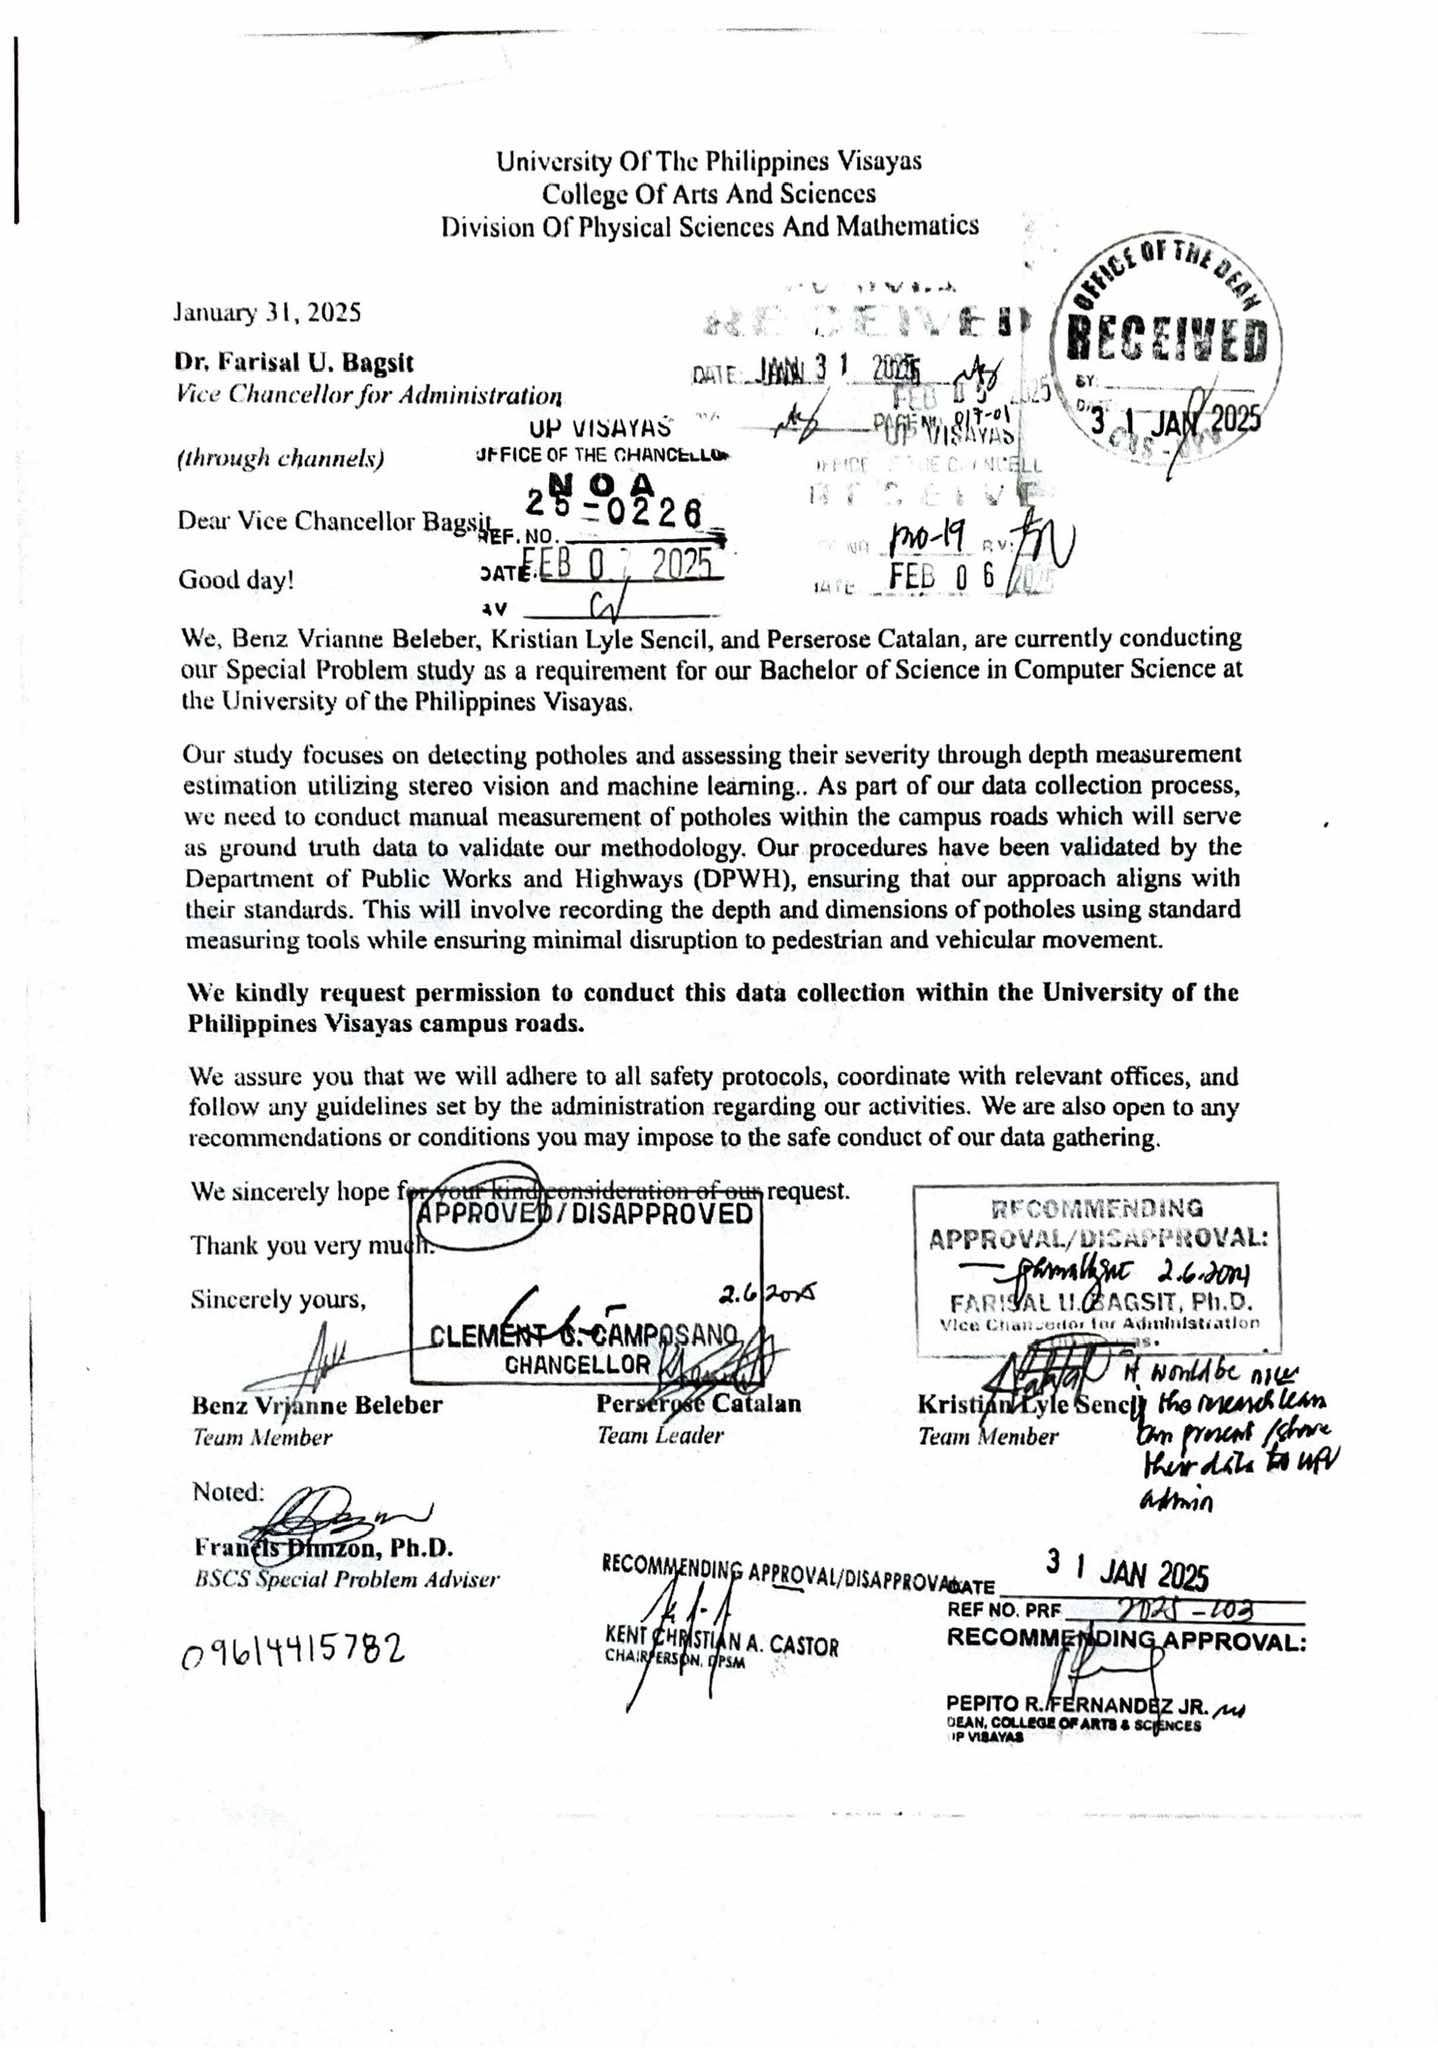
\includegraphics[width=\textwidth]{Admin_Letter.jpg}
	\caption{Letter requesting permission for ground truth data collection within the UPV campus.}
	\label{fig:permission_letter}
\end{figure}

\begin{figure}[htbp]
	\centering
	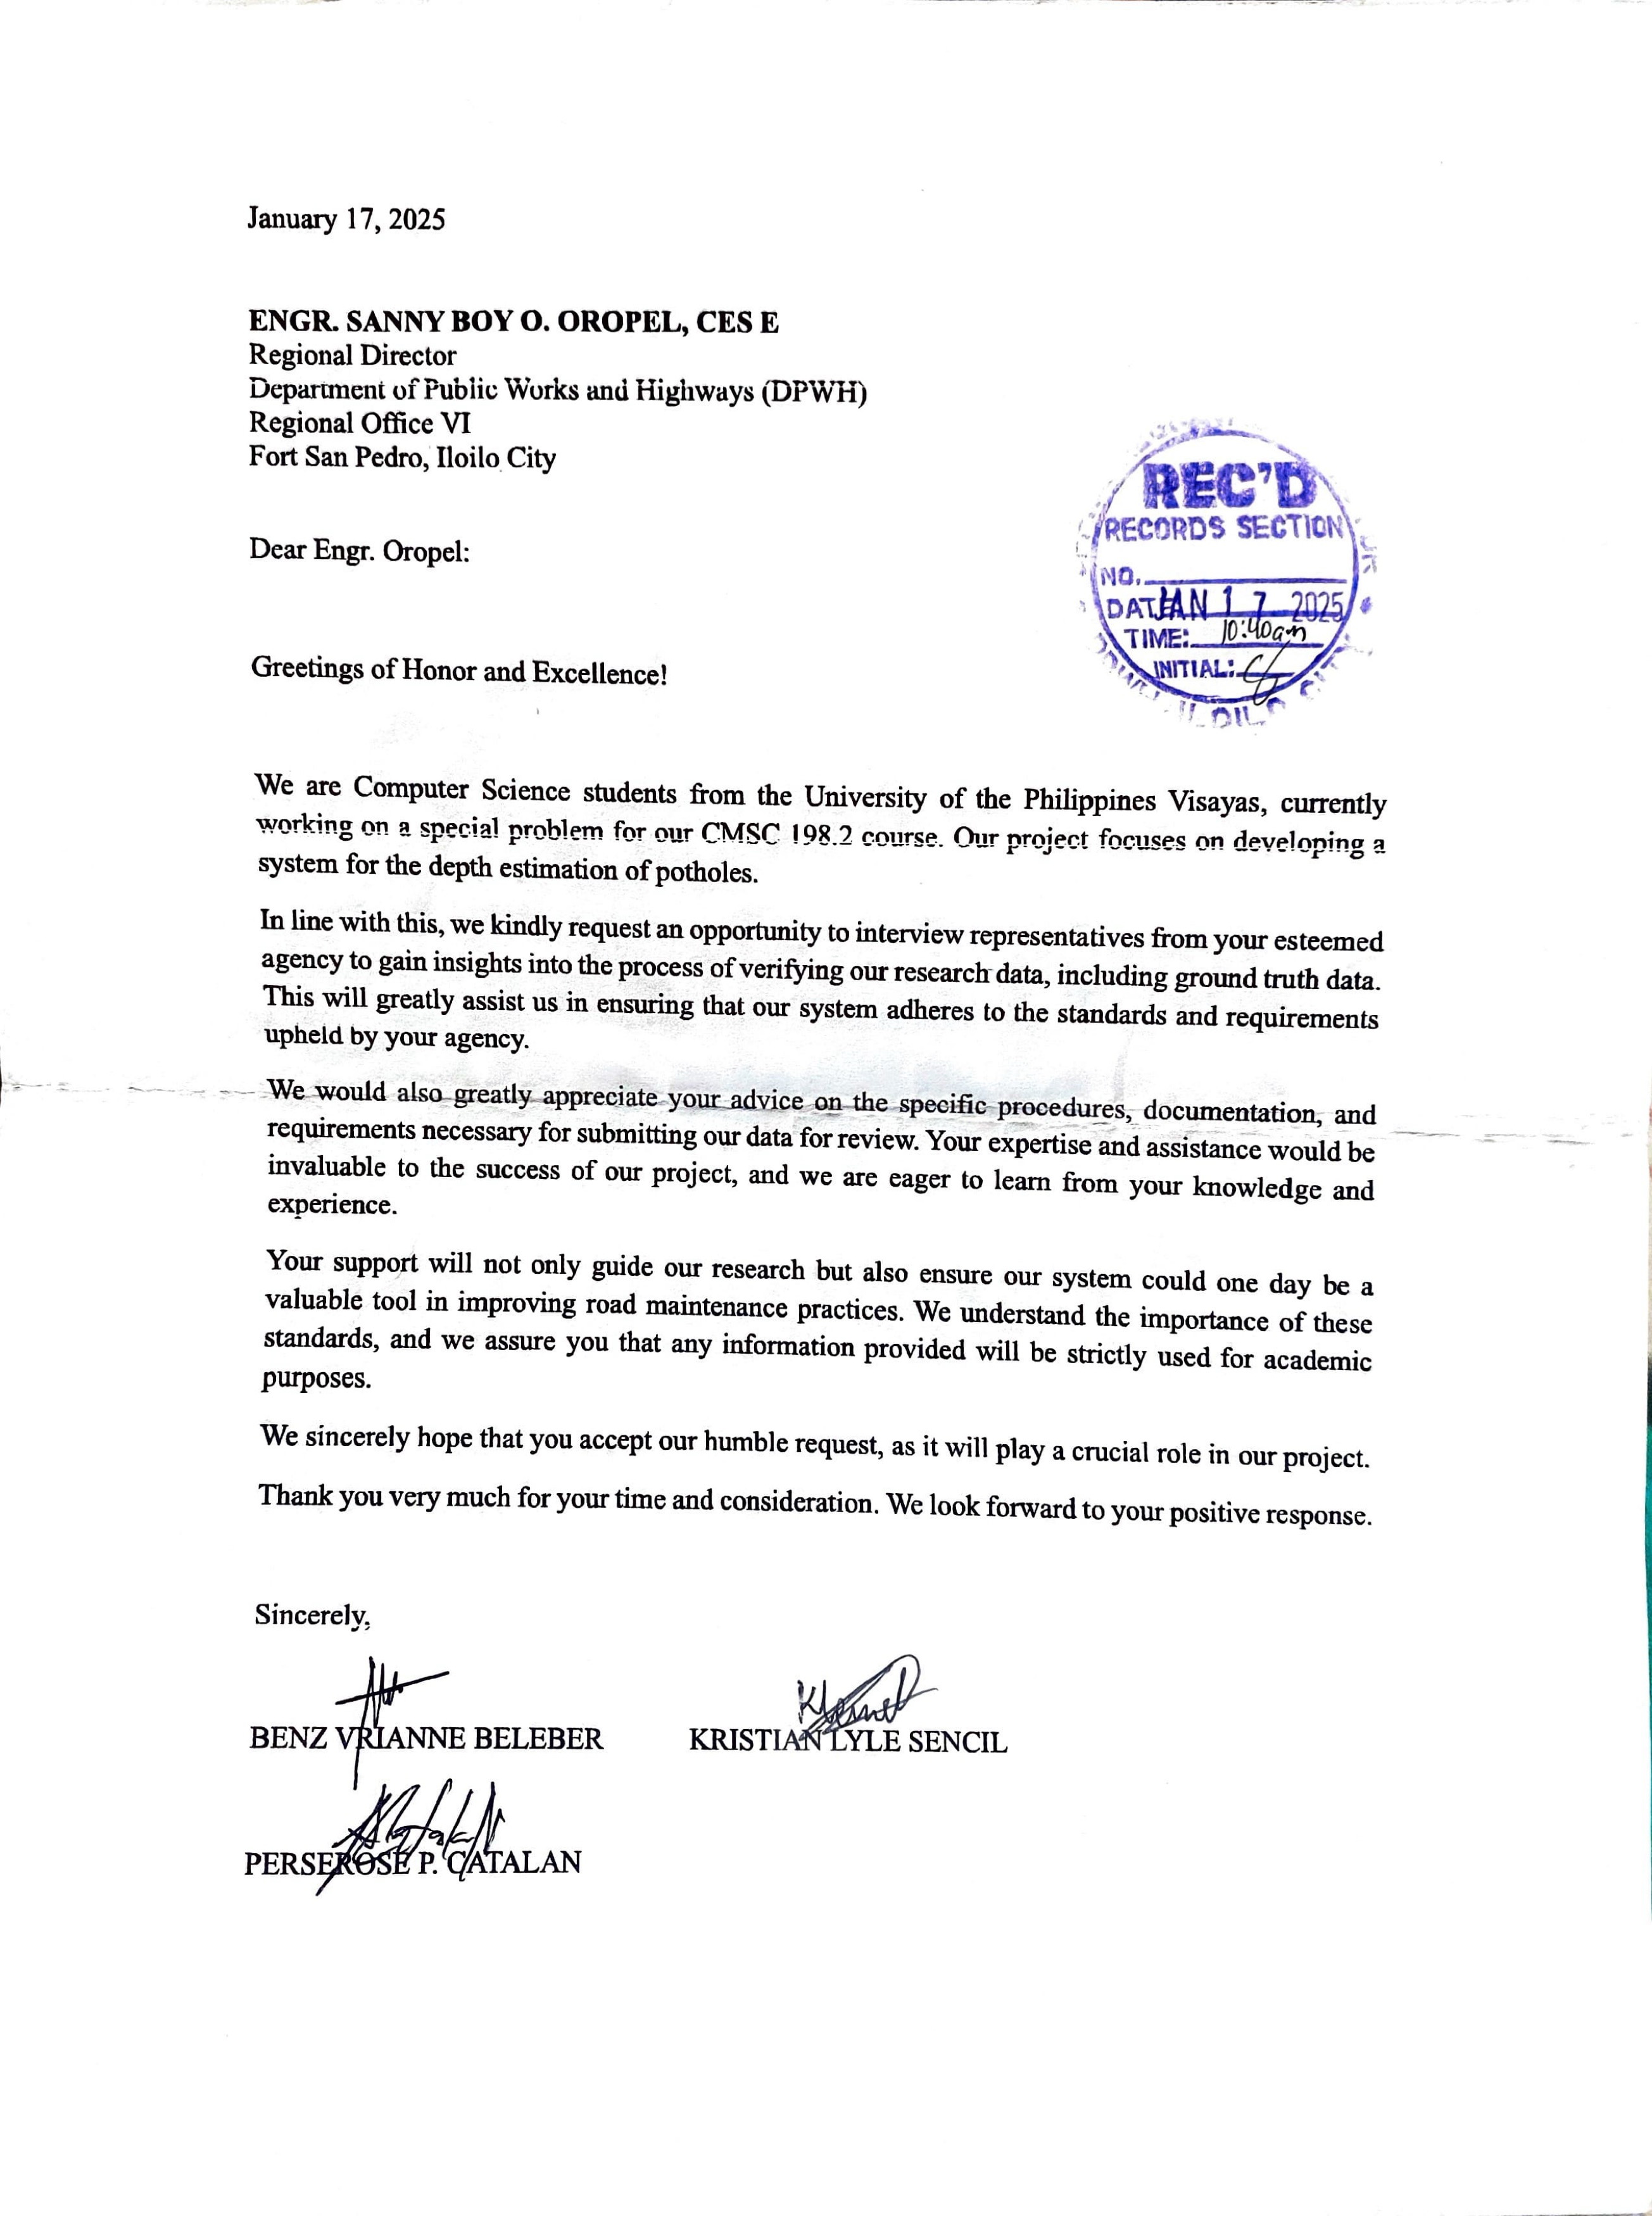
\includegraphics[width=\textwidth]{DPWH_Region.jpg}
	\caption{Letter requesting an interview with DPWH representatives for the process of verifying ground truth data.}
	\label{fig:regional_letter}
\end{figure}

\begin{figure}[htbp]
	\centering
	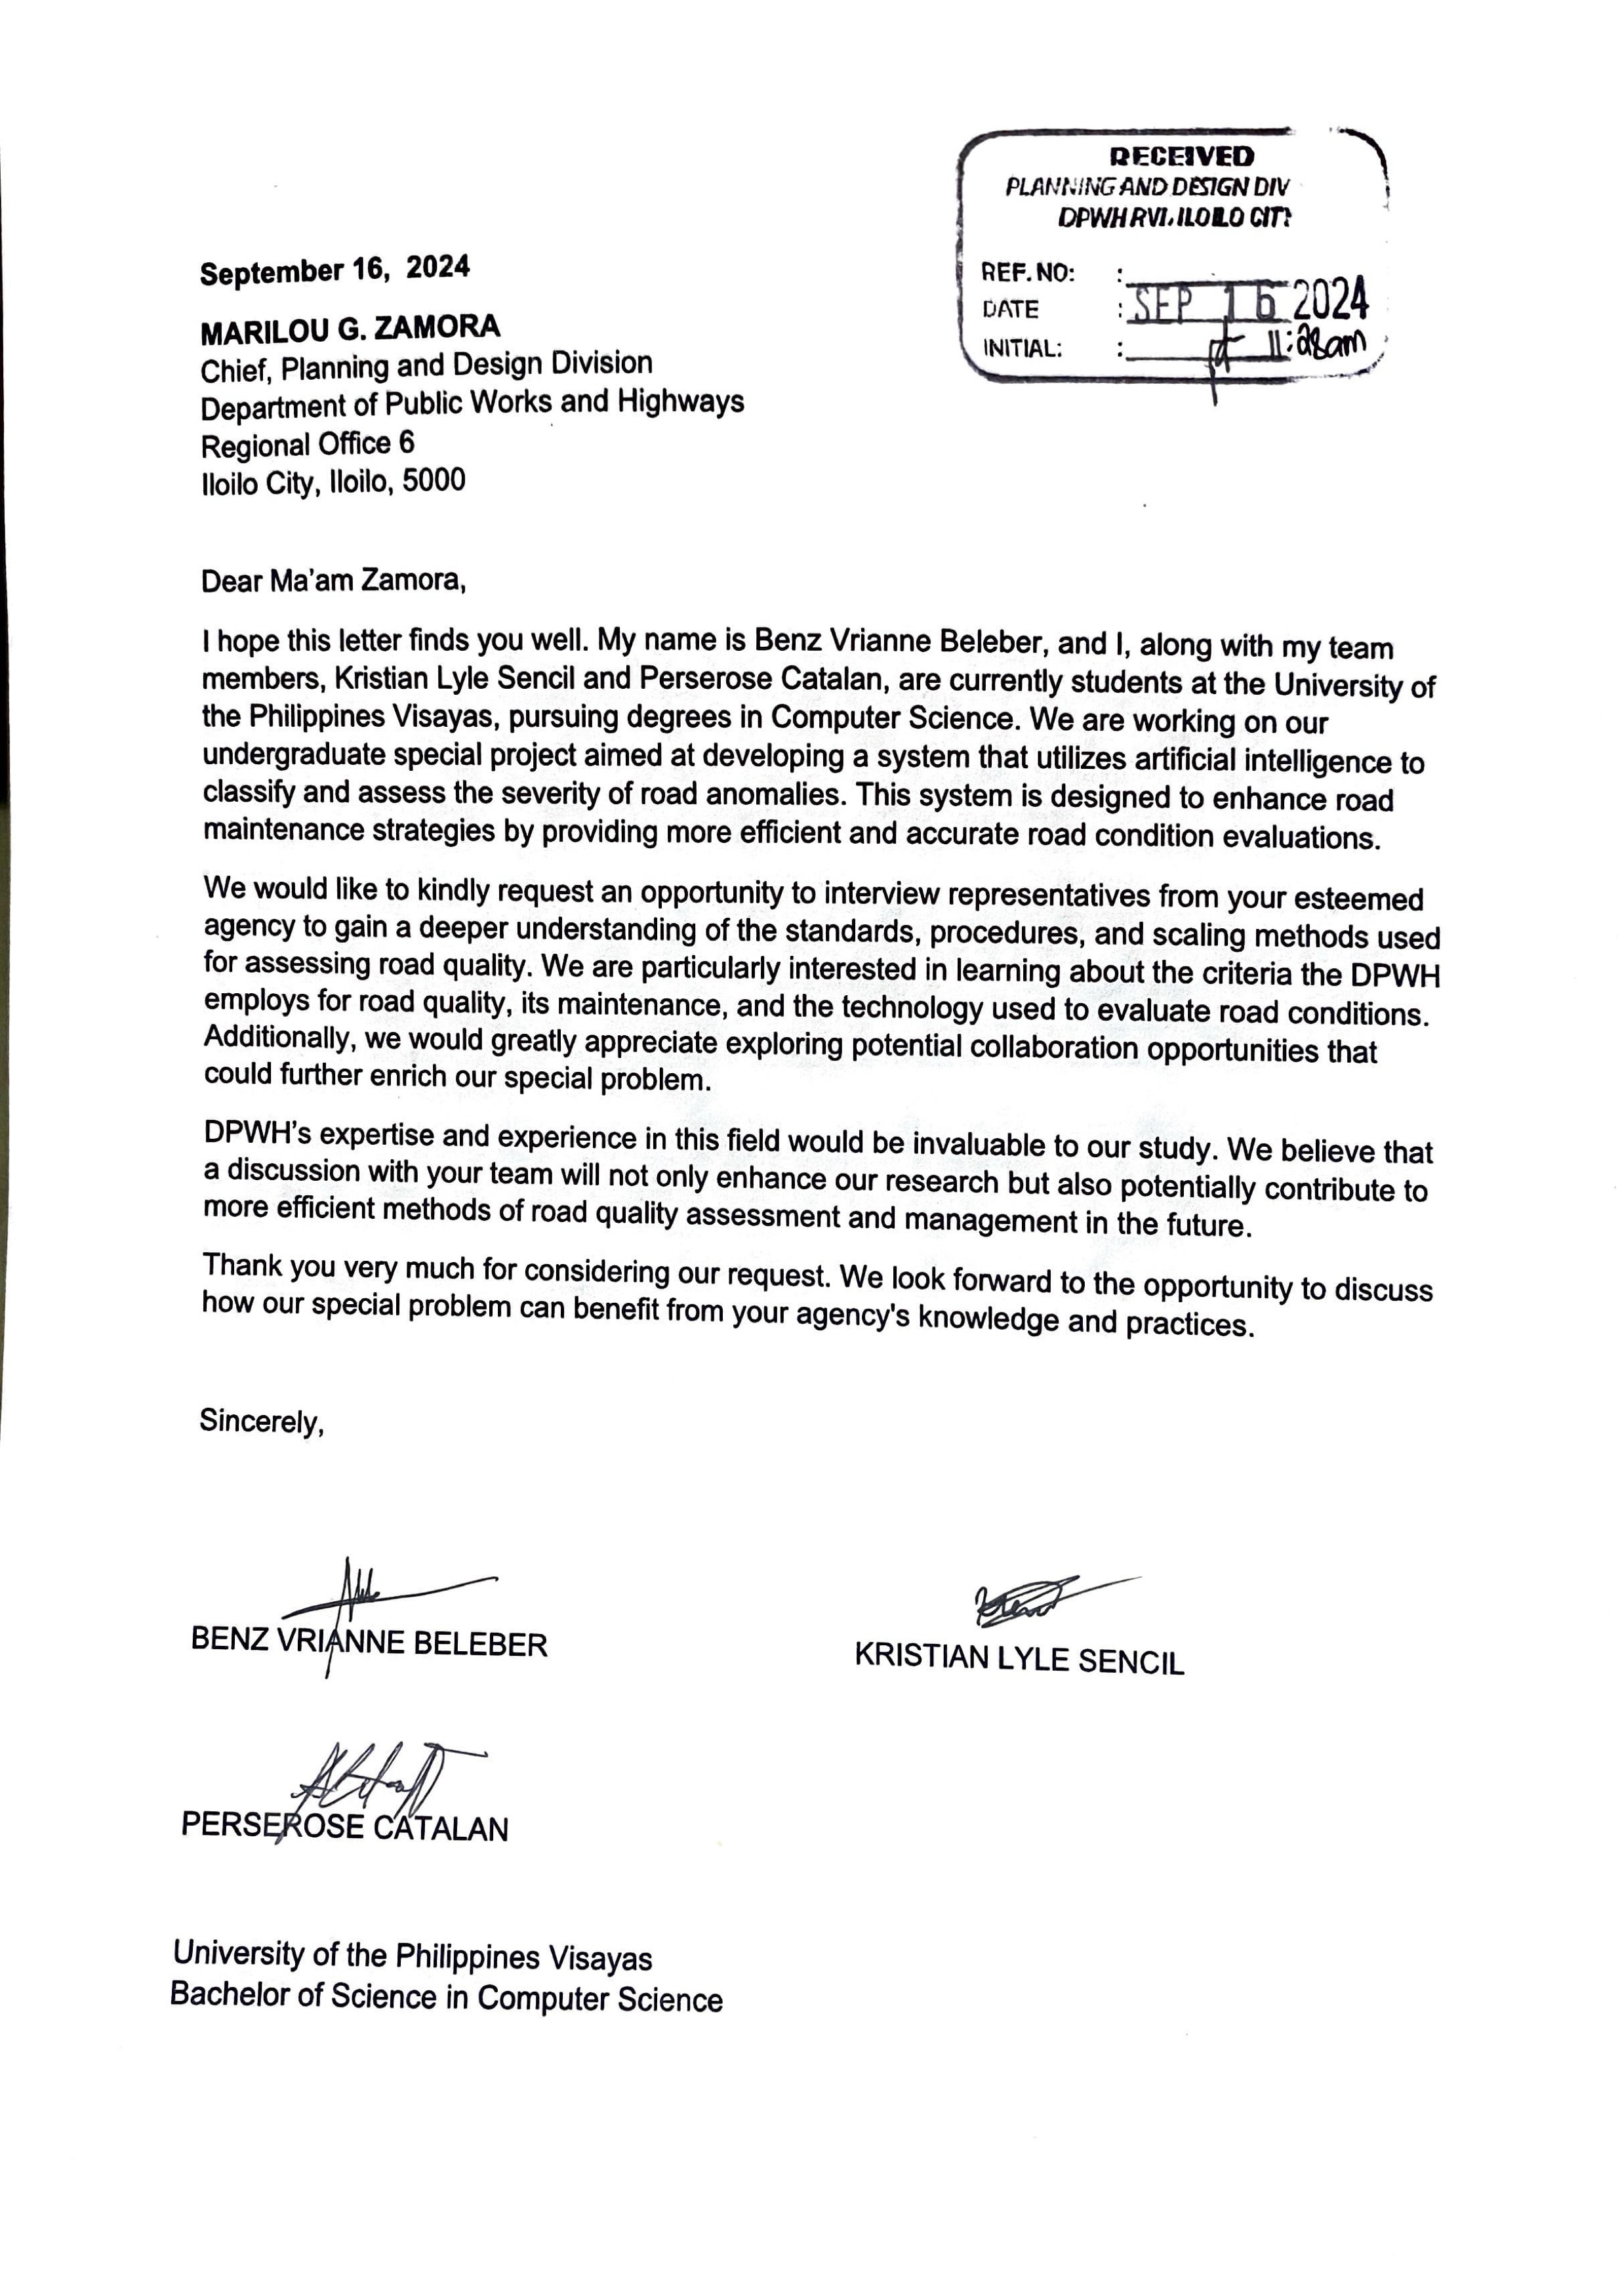
\includegraphics[width=\textwidth]{DPWH_First.jpg}
	\caption{Letter requesting an interview with DPWH representatives for the standard operating procedures of the agency for assessing road quality.}
	\label{fig:interview_letter}
\end{figure}

\begin{figure}[htbp]
	\centering
	
\includegraphics[width=\textwidth]{Manual_Page1.png}
	\caption{Validated pothole measurement procedural manual, reviewed by Engr. Ethel B. Morales, District Engineer, DPWH 1st District Engineering Office.}
	\label{fig:manual_page1}
\end{figure}

\begin{figure}[htbp]
	\centering
	
\includegraphics[width=\textwidth]{Manual_Page2.jpg}
	\caption{Second page of the pothole measurement procedural manual}
	\label{fig:manual_page2}
\end{figure}

\begin{figure}[htbp]
	\centering
	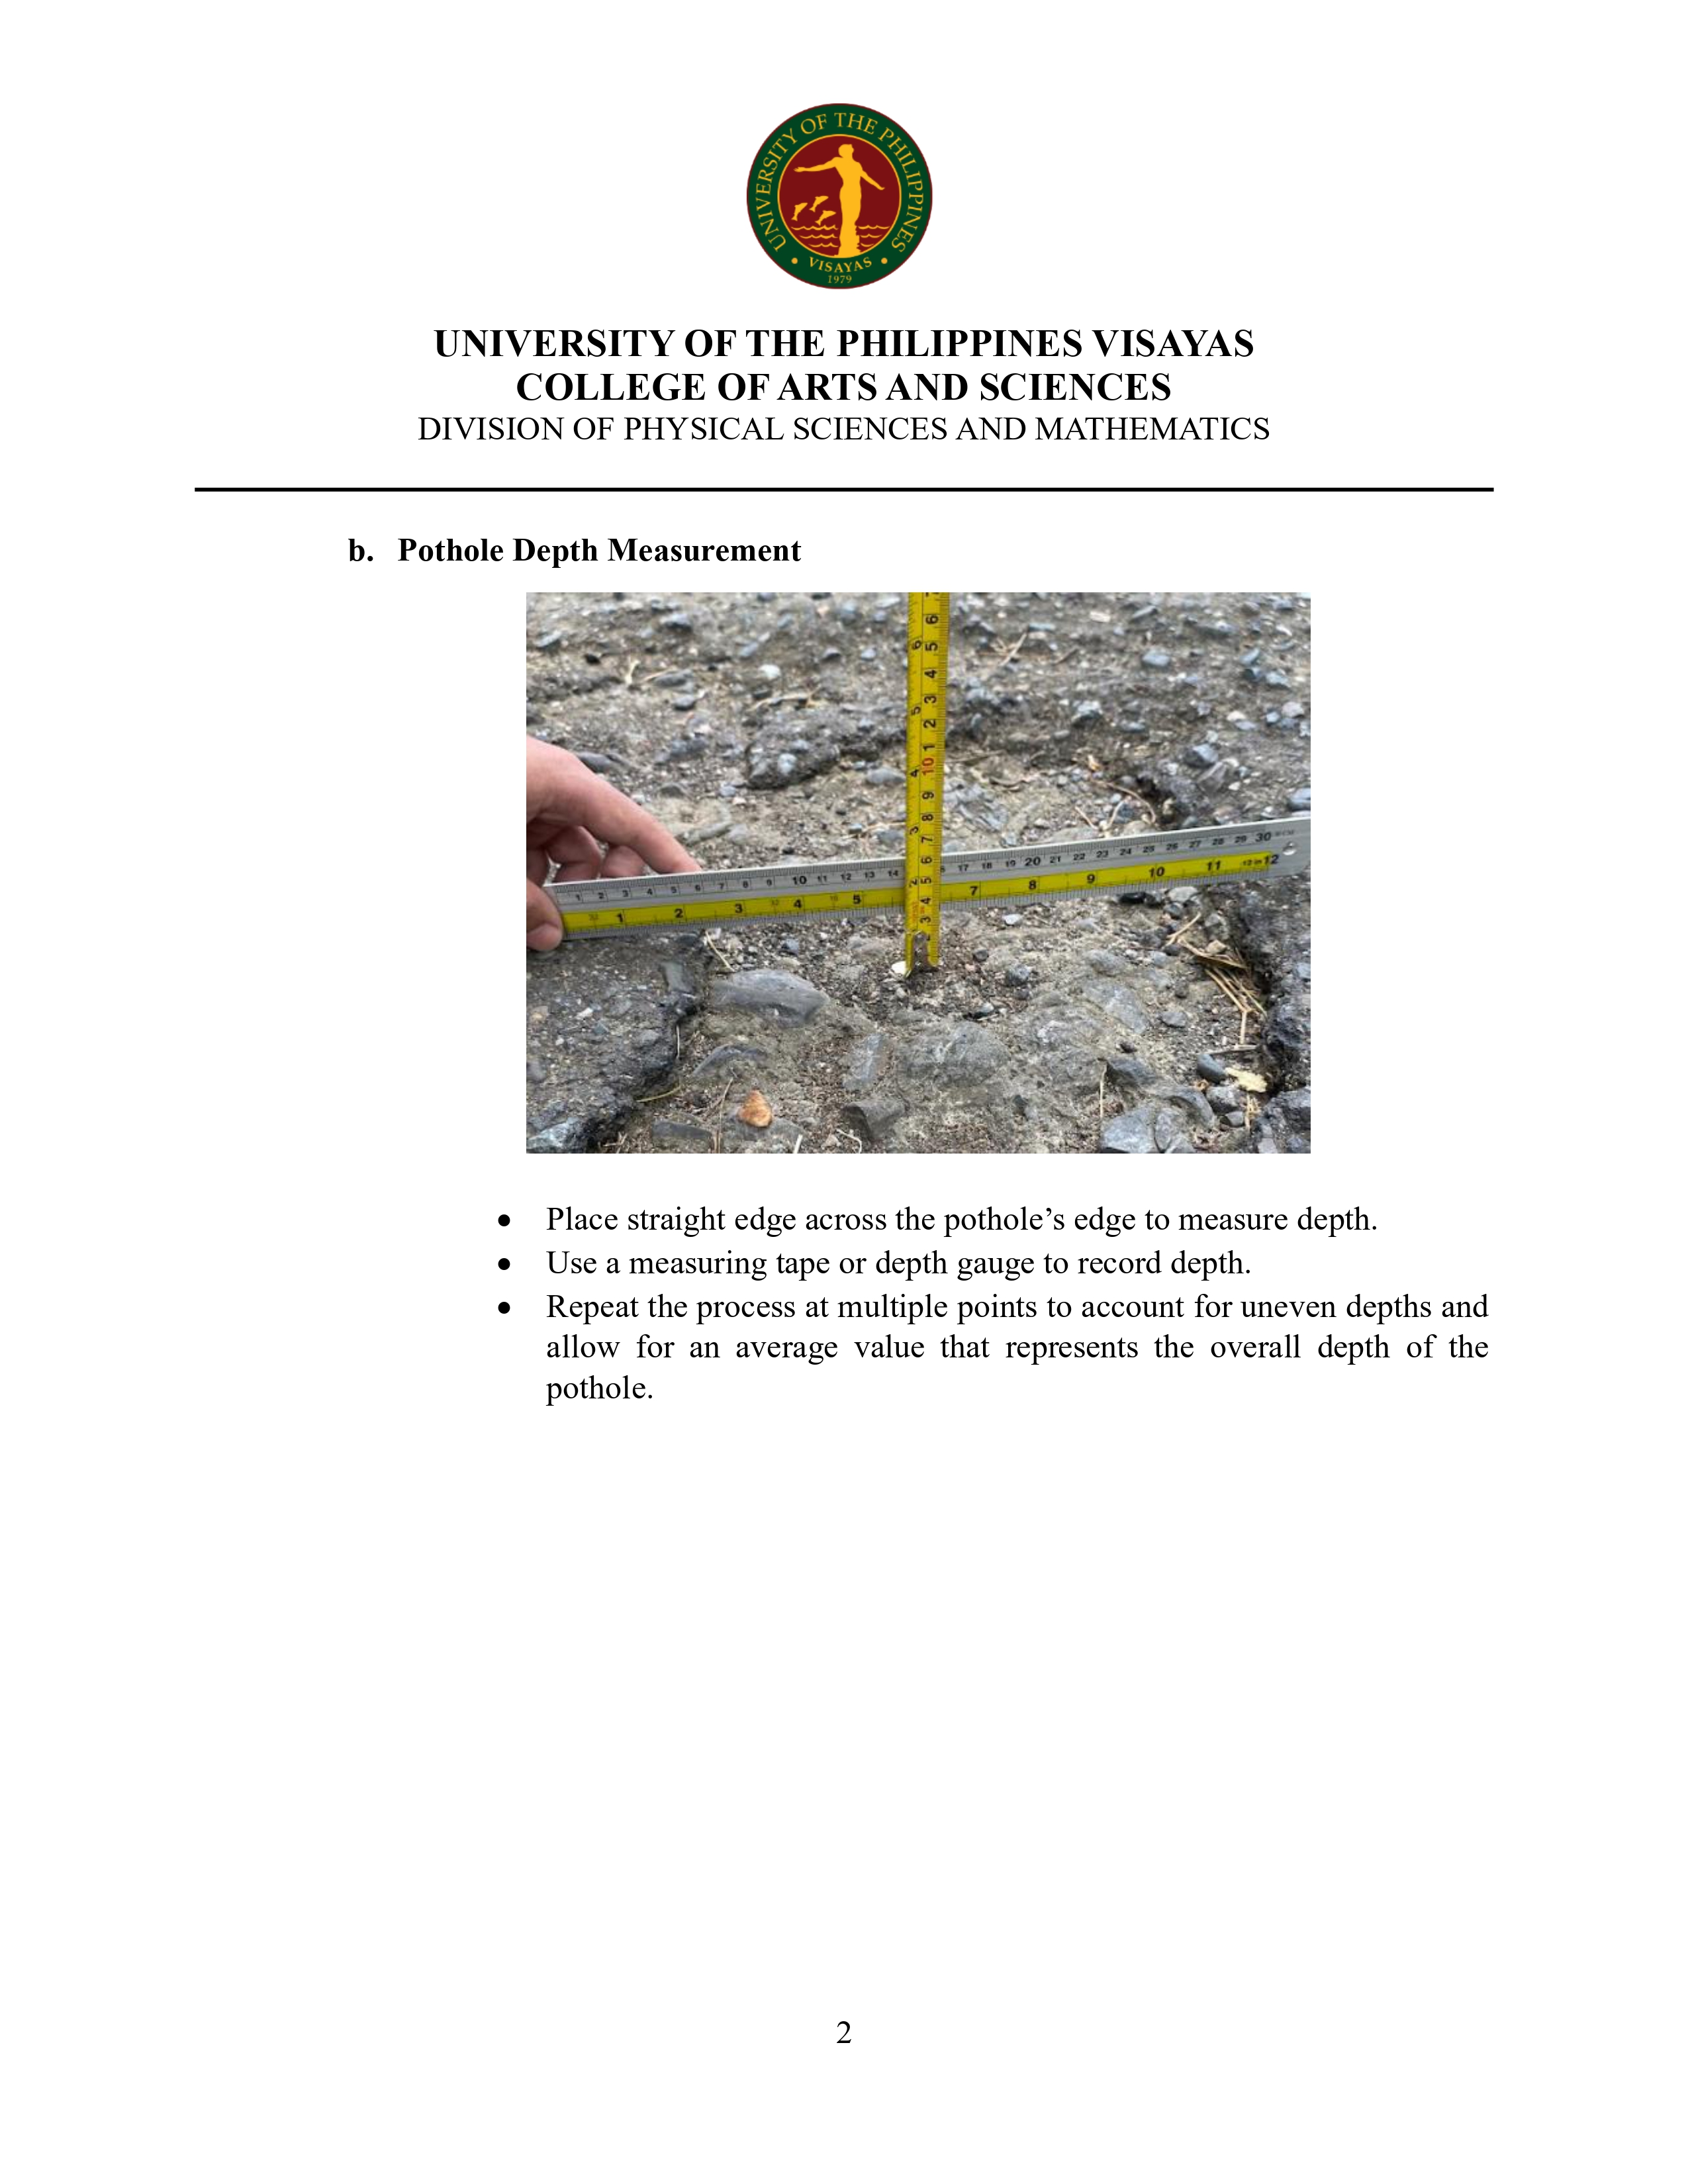
\includegraphics[width=\textwidth]{Manual_Page3.jpg}
	\caption{Third page of the pothole measurement procedural manual}
	\label{fig:manual_page3}
\end{figure}

\begin{figure}[htbp]
	\centering
	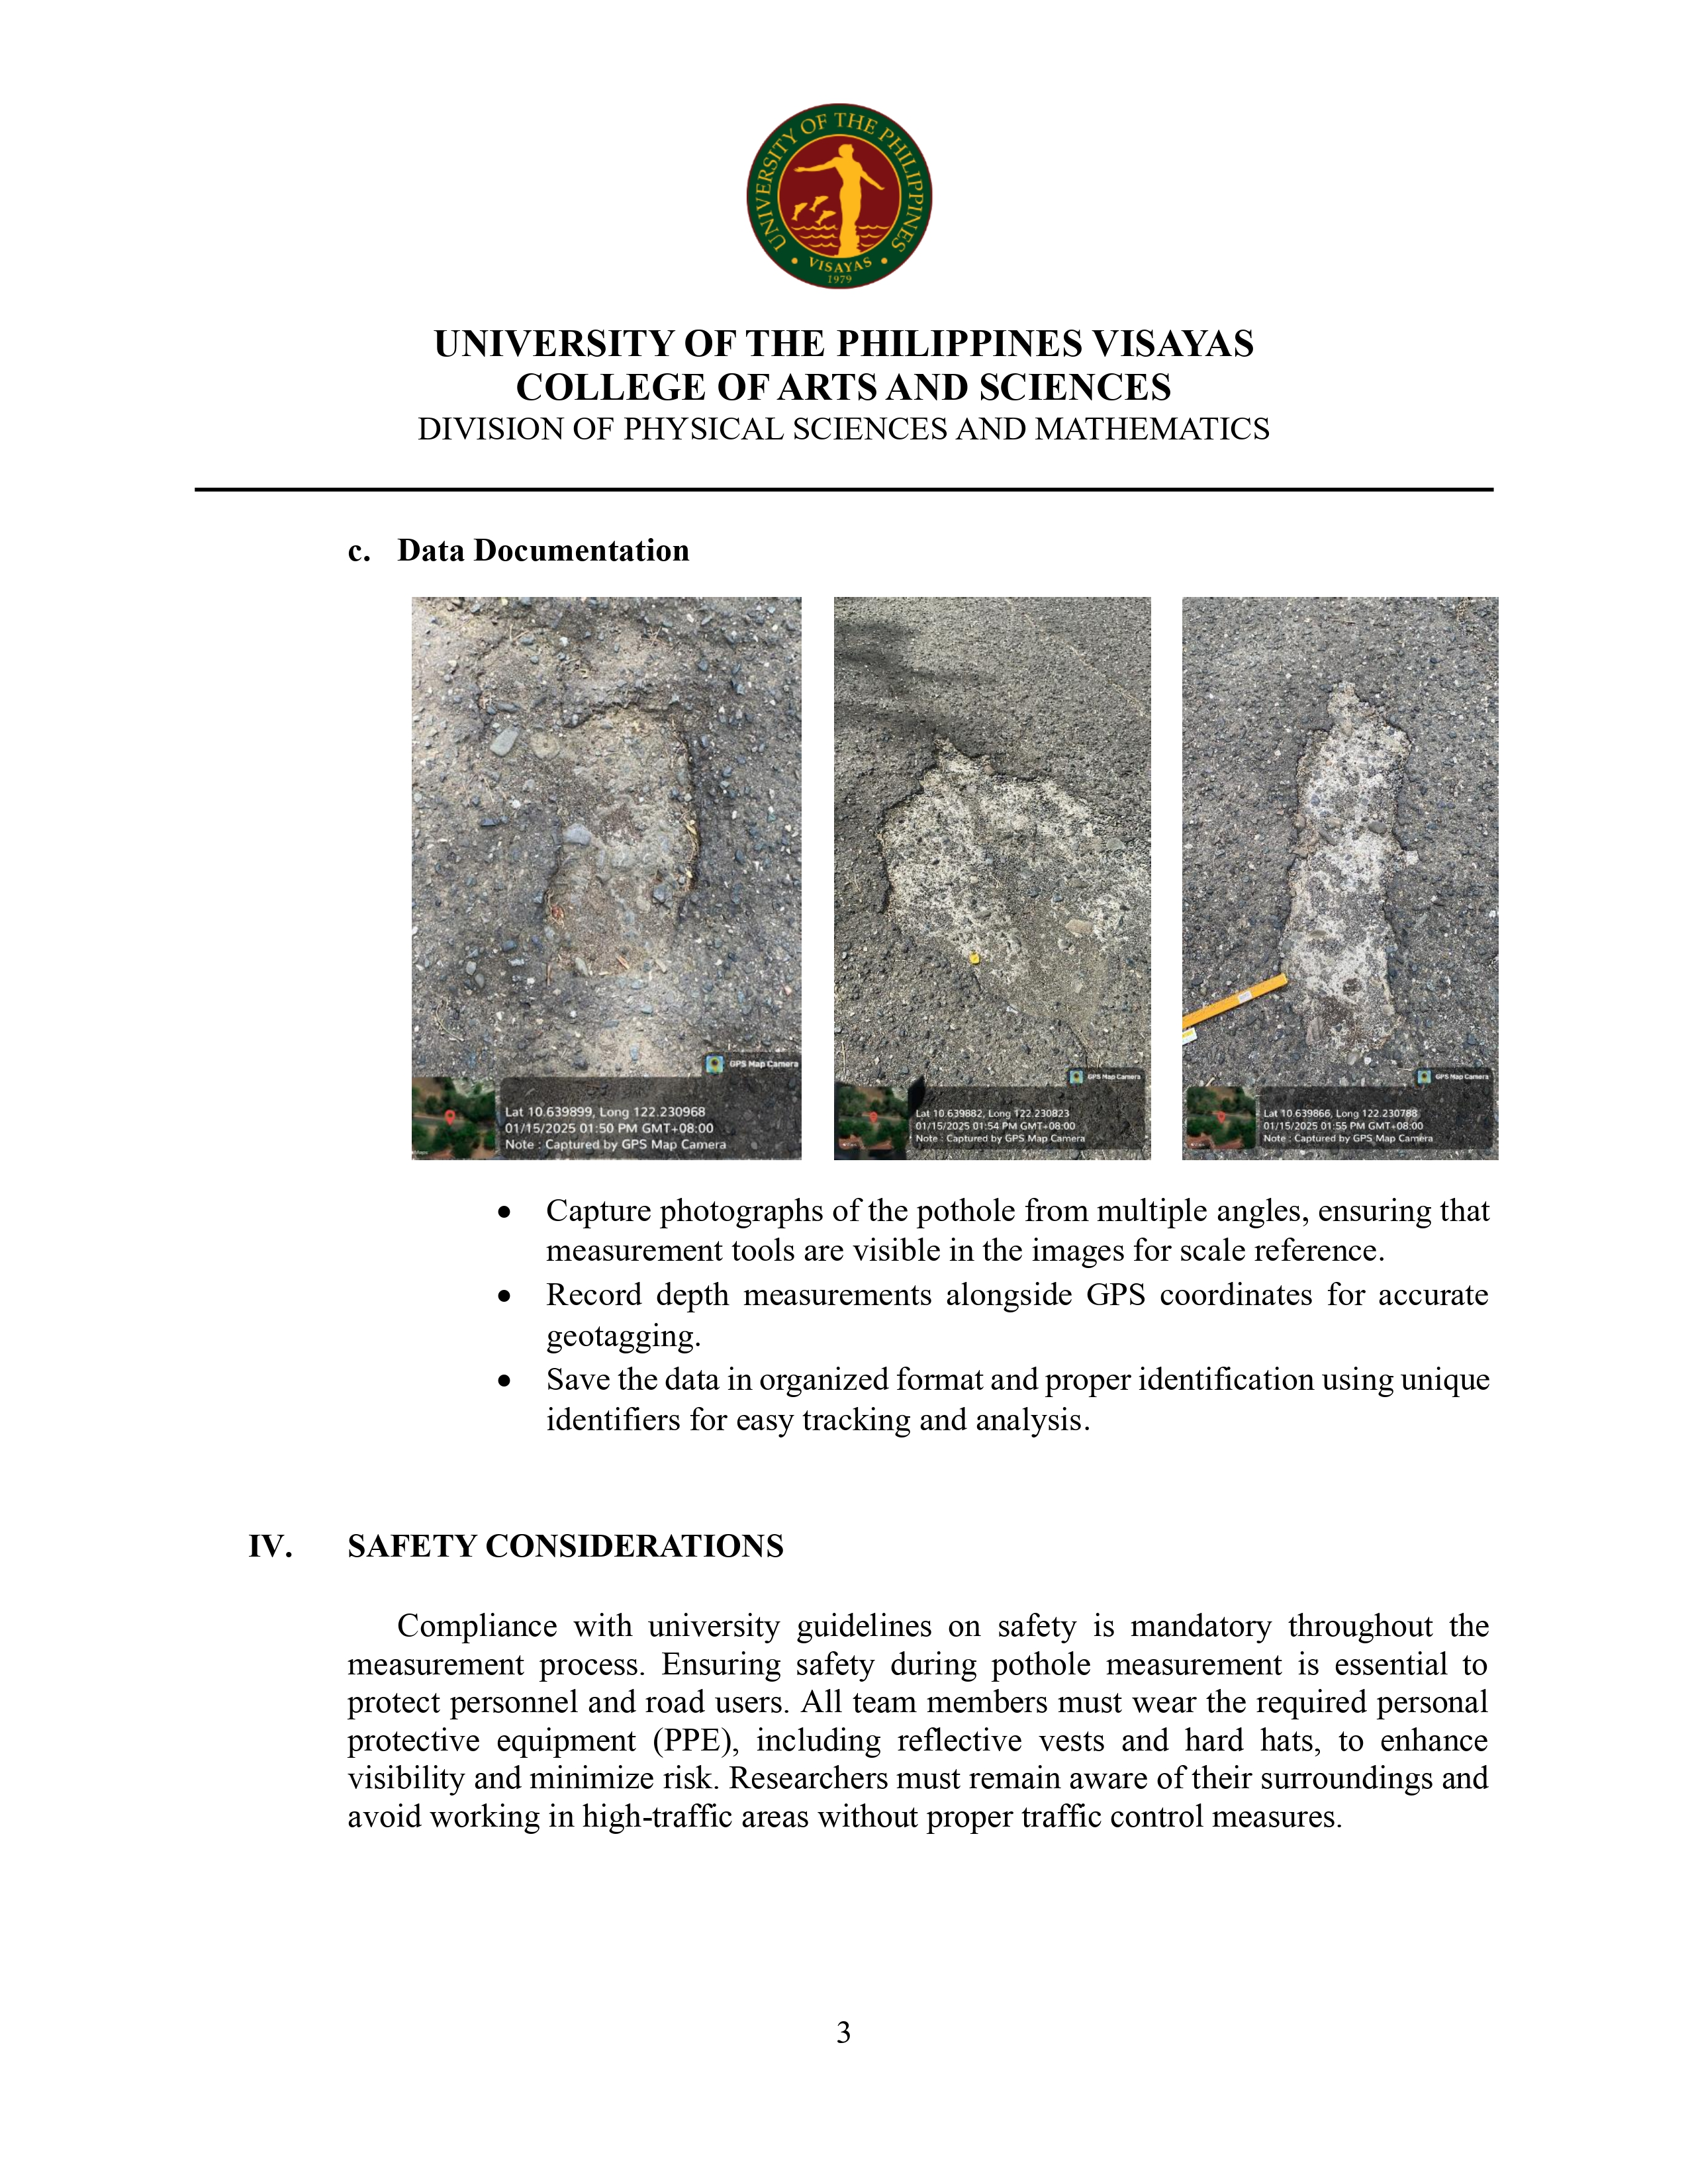
\includegraphics[width=\textwidth]{Manual_Page4.jpg}
	\caption{Fourth page of the pothole measurement procedural manual}
	\label{fig:manual_page4}
\end{figure}

\begin{figure}[htbp]
	\centering
	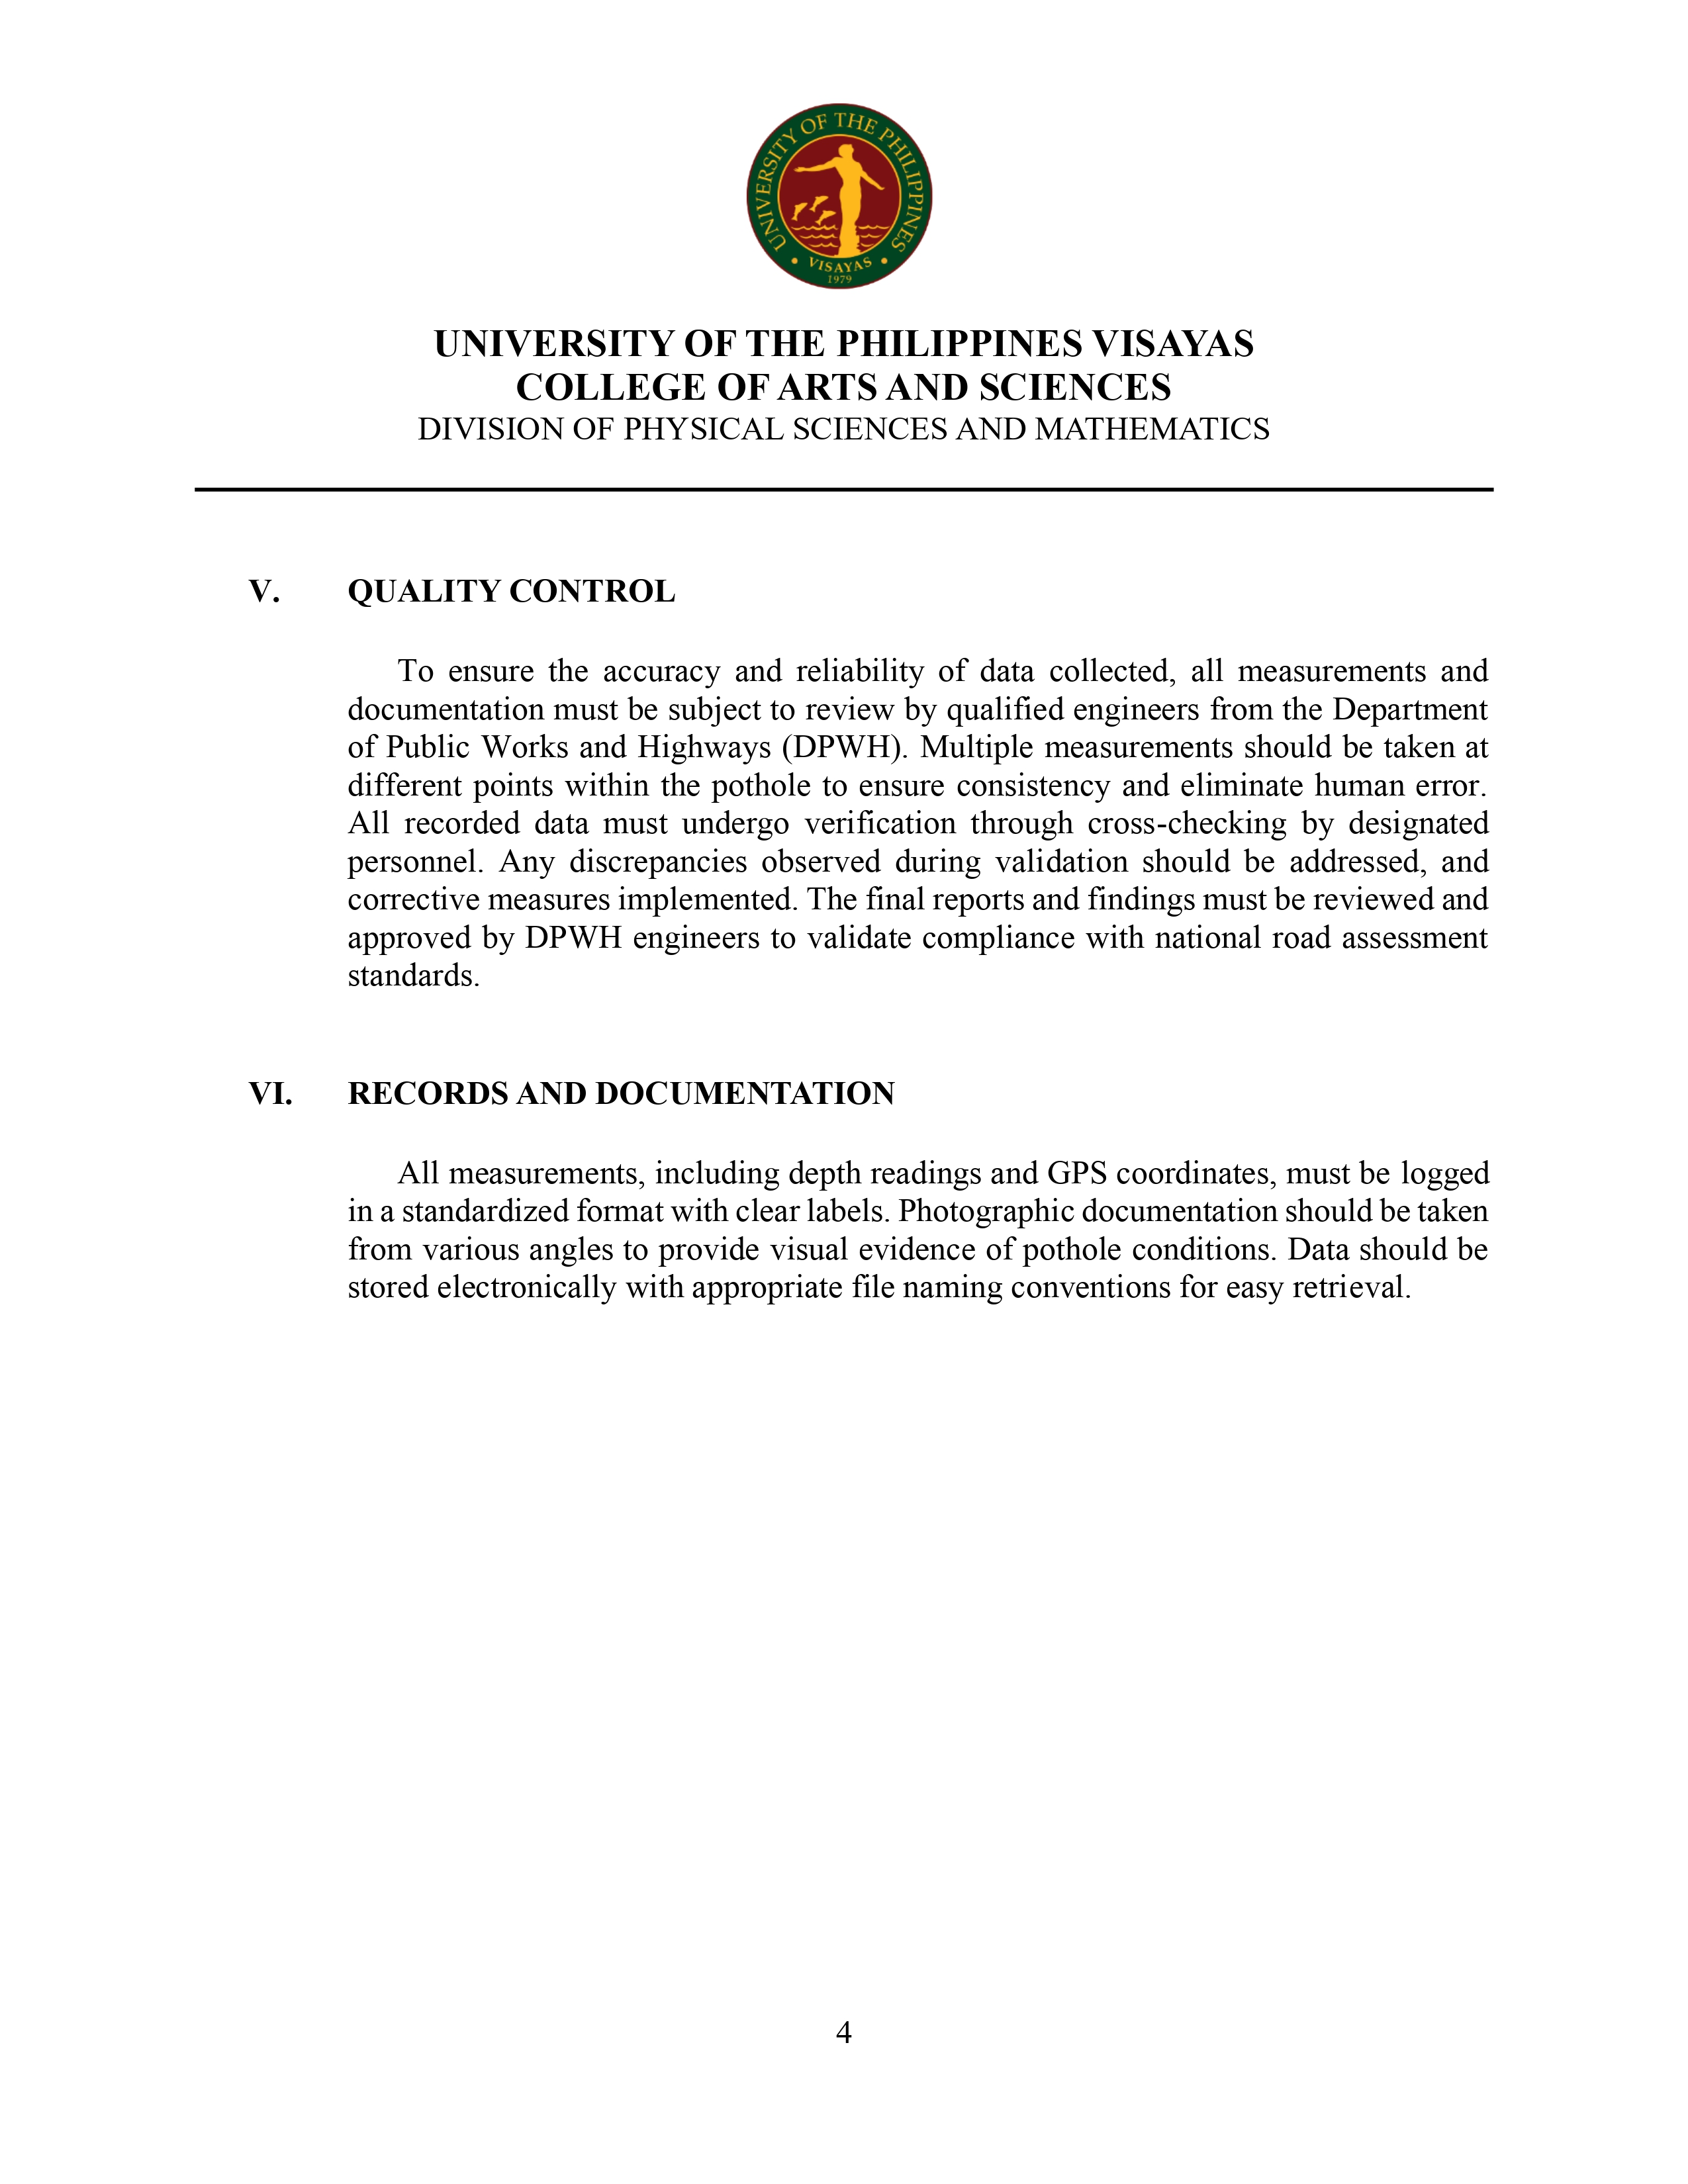
\includegraphics[width=\textwidth]{Manual_Page5.jpg}
	\caption{Fifth page of the pothole measurement procedural manual}
	\label{fig:manual_page5}
\end{figure}


              %LaTeX source file for Appendix D


\end{document}

